\documentclass[letterpaper,14pt,titlepage,fleqn]{article}

\setlength{\mathindent}{1cm}

\usepackage{graphicx}                                        

\usepackage{amssymb}                                         
\usepackage{amsmath}                                         
\usepackage{amsthm}                                          

\usepackage{alltt}                                           
\usepackage{float}
\usepackage{color}

\usepackage{url}

\usepackage{balance}
\usepackage[TABBOTCAP, tight]{subfigure}
\usepackage{enumitem}

\usepackage{pstricks, pst-node}

\usepackage{cite}
\usepackage{indentfirst}
\usepackage{listings}

% the following sets the geometry of the page
\usepackage{geometry}
\geometry{textheight=9in, textwidth=6.5in}

% random comment

\newcommand{\cred}[1]{{\color{red}#1}}
\newcommand{\cblue}[1]{{\color{blue}#1}}

\usepackage{hyperref}

\usepackage{textcomp}
\usepackage{listings}

\def\name{Haoxiang Wang; Student ID: 932359049}

%% The following metadata will show up in the PDF properties
\hypersetup{
  colorlinks = true,
  urlcolor = black,
  pdfauthor = {\name},
  pdfkeywords = {CS557 Project 7},
  pdftitle = {Project \#7: A Tessellated Parametric Triangular B\'{e}zier Patch},
  pdfsubject = {Project \#7: A Tessellated Parametric Triangular B\'{e}zier Patch},
  pdfpagemode = UseNone
}

\parindent = 0.0 in
\parskip = 0.2 in

\author{\name}
\title{Project \#7: A Tessellated Parametric Triangular B\'{e}zier Patch}

\begin{document}
\maketitle

This project is the Seventh project I have done in this class, and it is the last project we have except the final. We are required to implement a triangular B\'{e}zier patch using tessellation shaders. This is the project contains most shader files but not the hardest to do. The whole project only takes me a few hours to implement since most part of the code has been given in the project description. The results images and the explanation of how code works will be described in the after section. 

\section{Source Listing}
In this project, six files are necessary. Except the .glib file, all other five files are shaders. This project contains vertex shader, tessellation shader, geometry shader and fragment shader. Vertex shader just passes vertex information out. Tessellation control shader transforms the input coordinates to a regular surface representation. Tessellation evaluation shader evaluates the surface in uvw coordinates. Geometry shader implements the 11shrink'' effect for triangles. Fragment shader mainly implements lighting. The specific filenames and usages are listed below.

mtriangle.glib --- Handle the user interface and object\\
mtriangle.vert --- Handle the vertex shader\\
mtriangle.tcs --- Handle tessellation control shader\\
mtriangle.tes --- Handle tessellation evaluation shader\\
mtriangle.geom --- Handle geometry shader\\
mtriangle.frag --- Handle the fragment shader\\

\section{Result Images and Explanation}
There are a bunch of shader files used in this project. The project also requires a lot features that control the scene. It has sliders control outer and inner densities, the height of each edge, how much the triangles shrink, and all of the lighting parameters. All of the features will be examined in the following paragraphs. The following image shows the origin look of the scene when the .glib file is loaded.
\begin{center}
	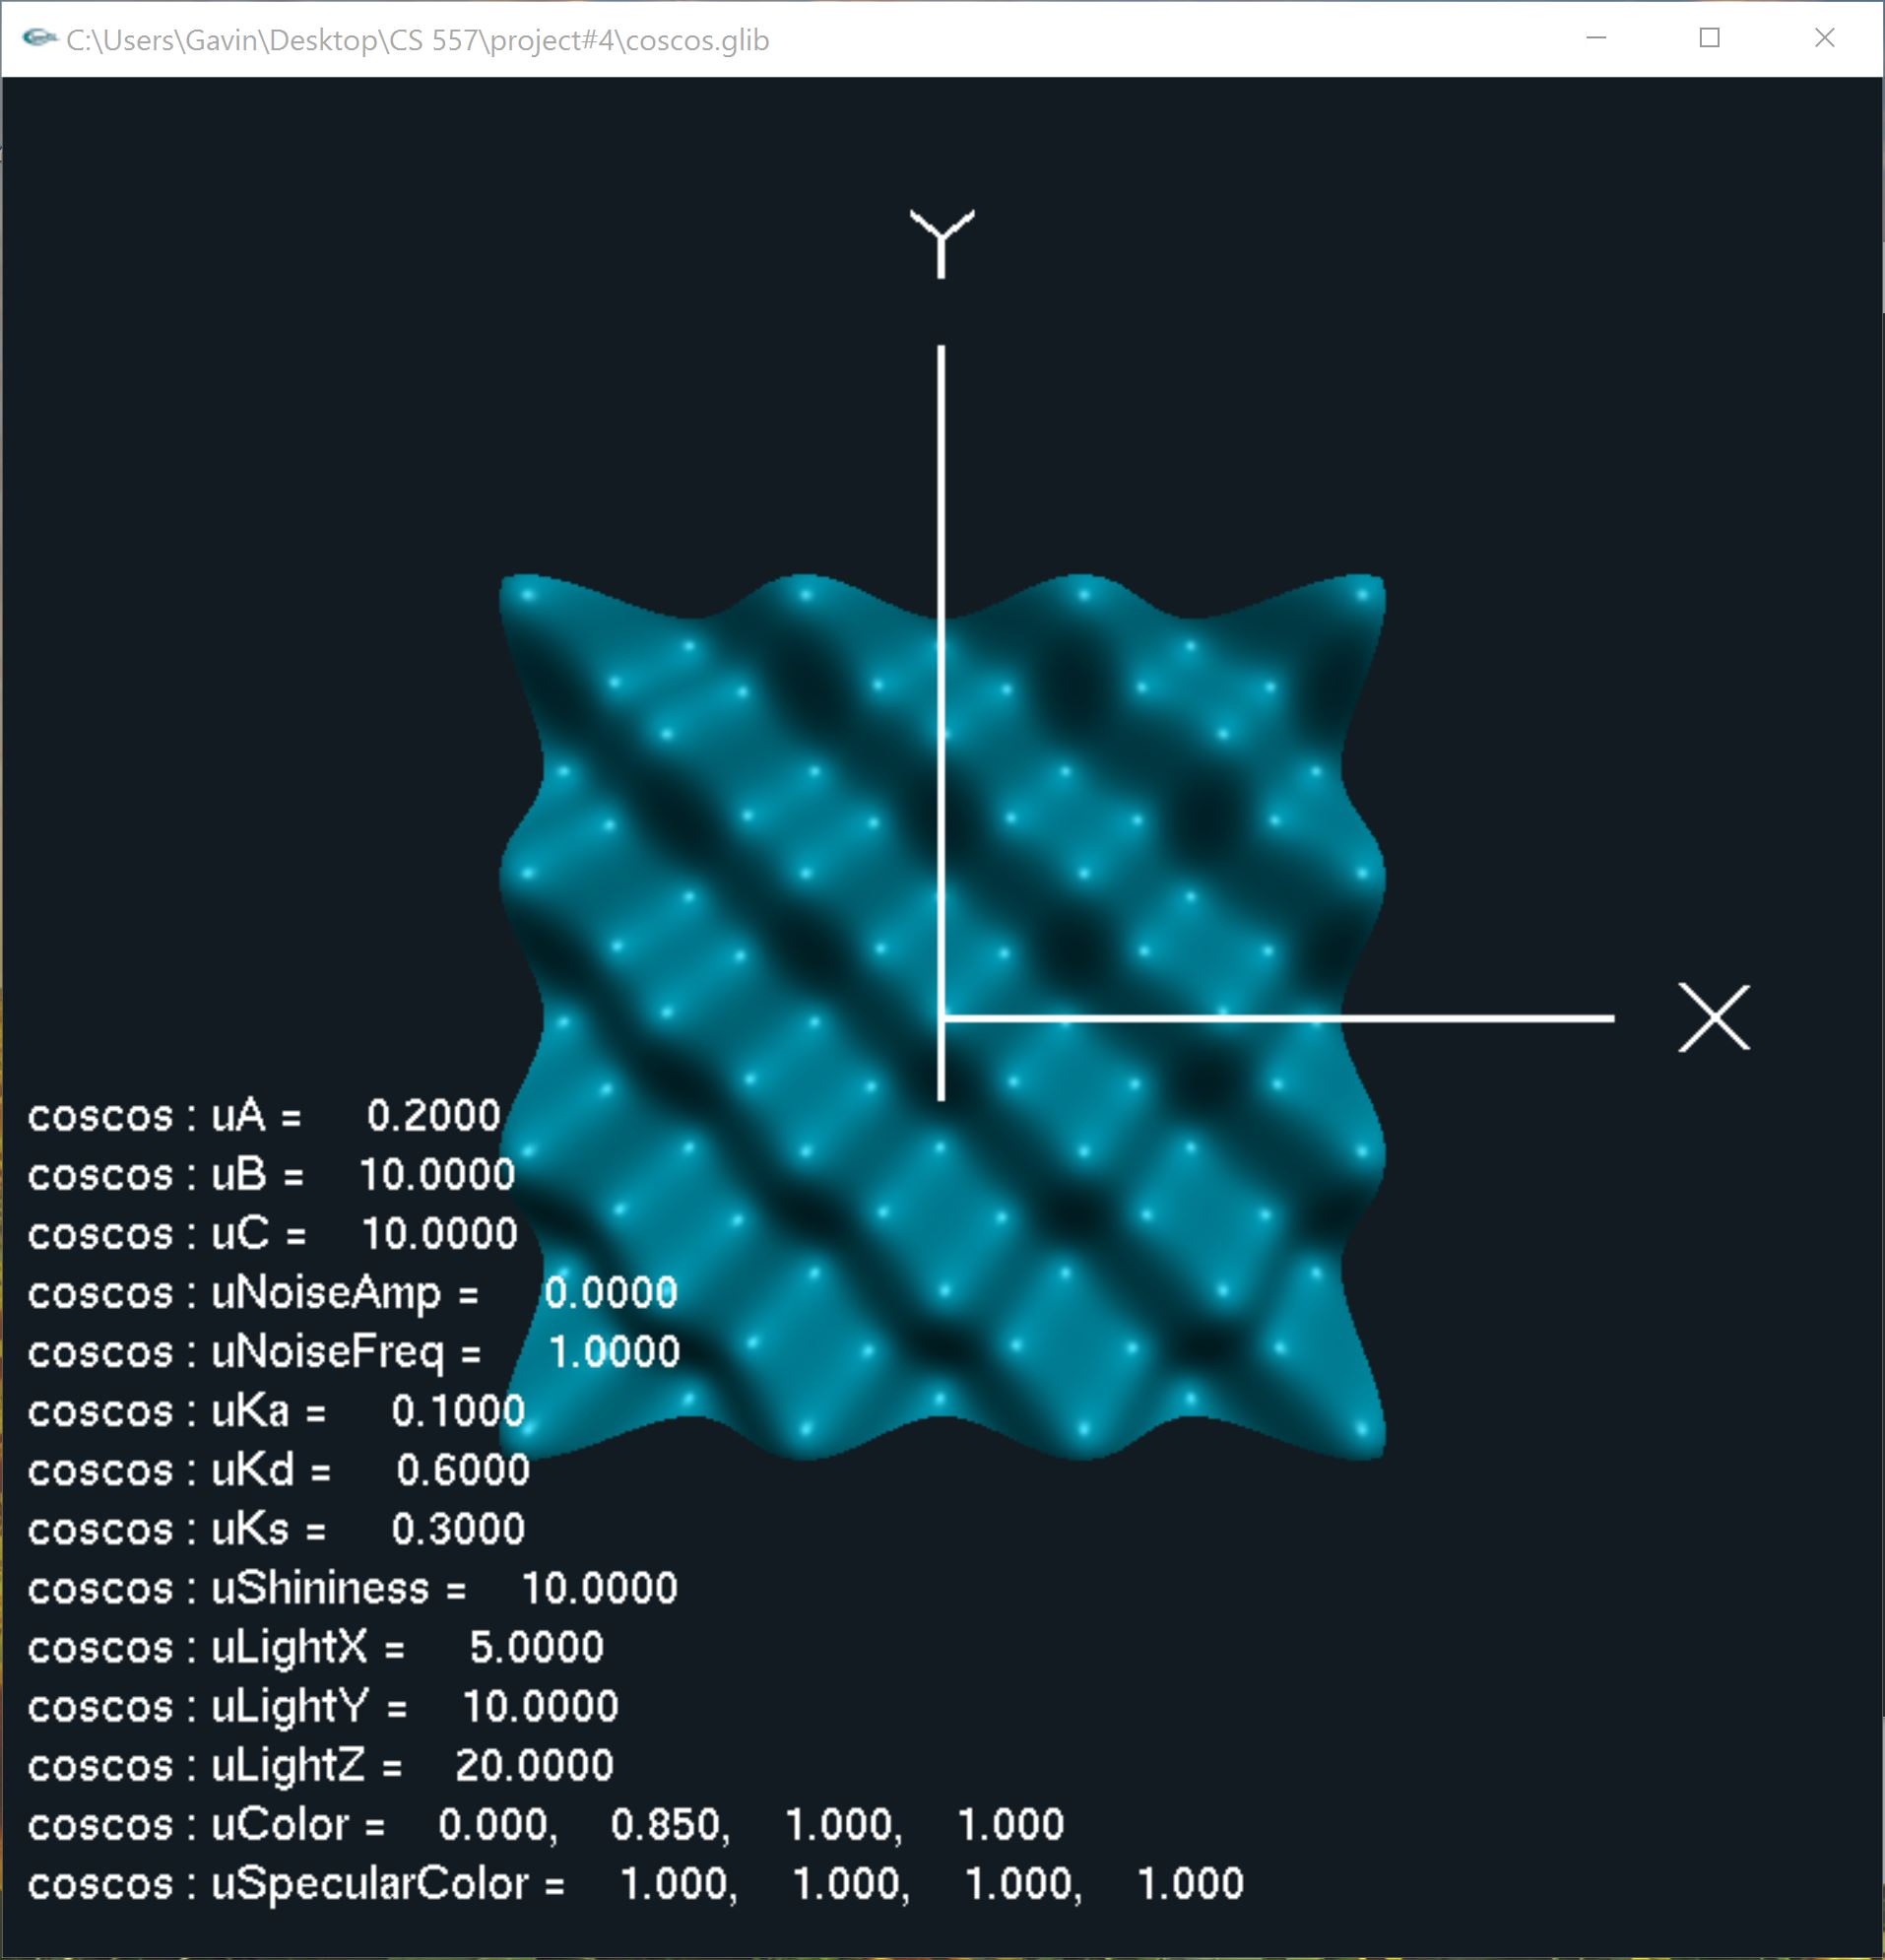
\includegraphics[width=2.8in]{origin.jpg}
\end{center}
In the original scene, the densities along each edge is set to one by default. The densities of inner part of the patch is also set to one by default. So the whole patch looks one solid triangle. the nymber of outer and inner densities are controlled by sliders. The following images shows the changes when the outer and inner sliders are changed. In the previous three images, the inner is set to 3, and three outer edges are set to 10 one by one. The fourth image has inner set to 10 with three outer remain 10.
\begin{center}
	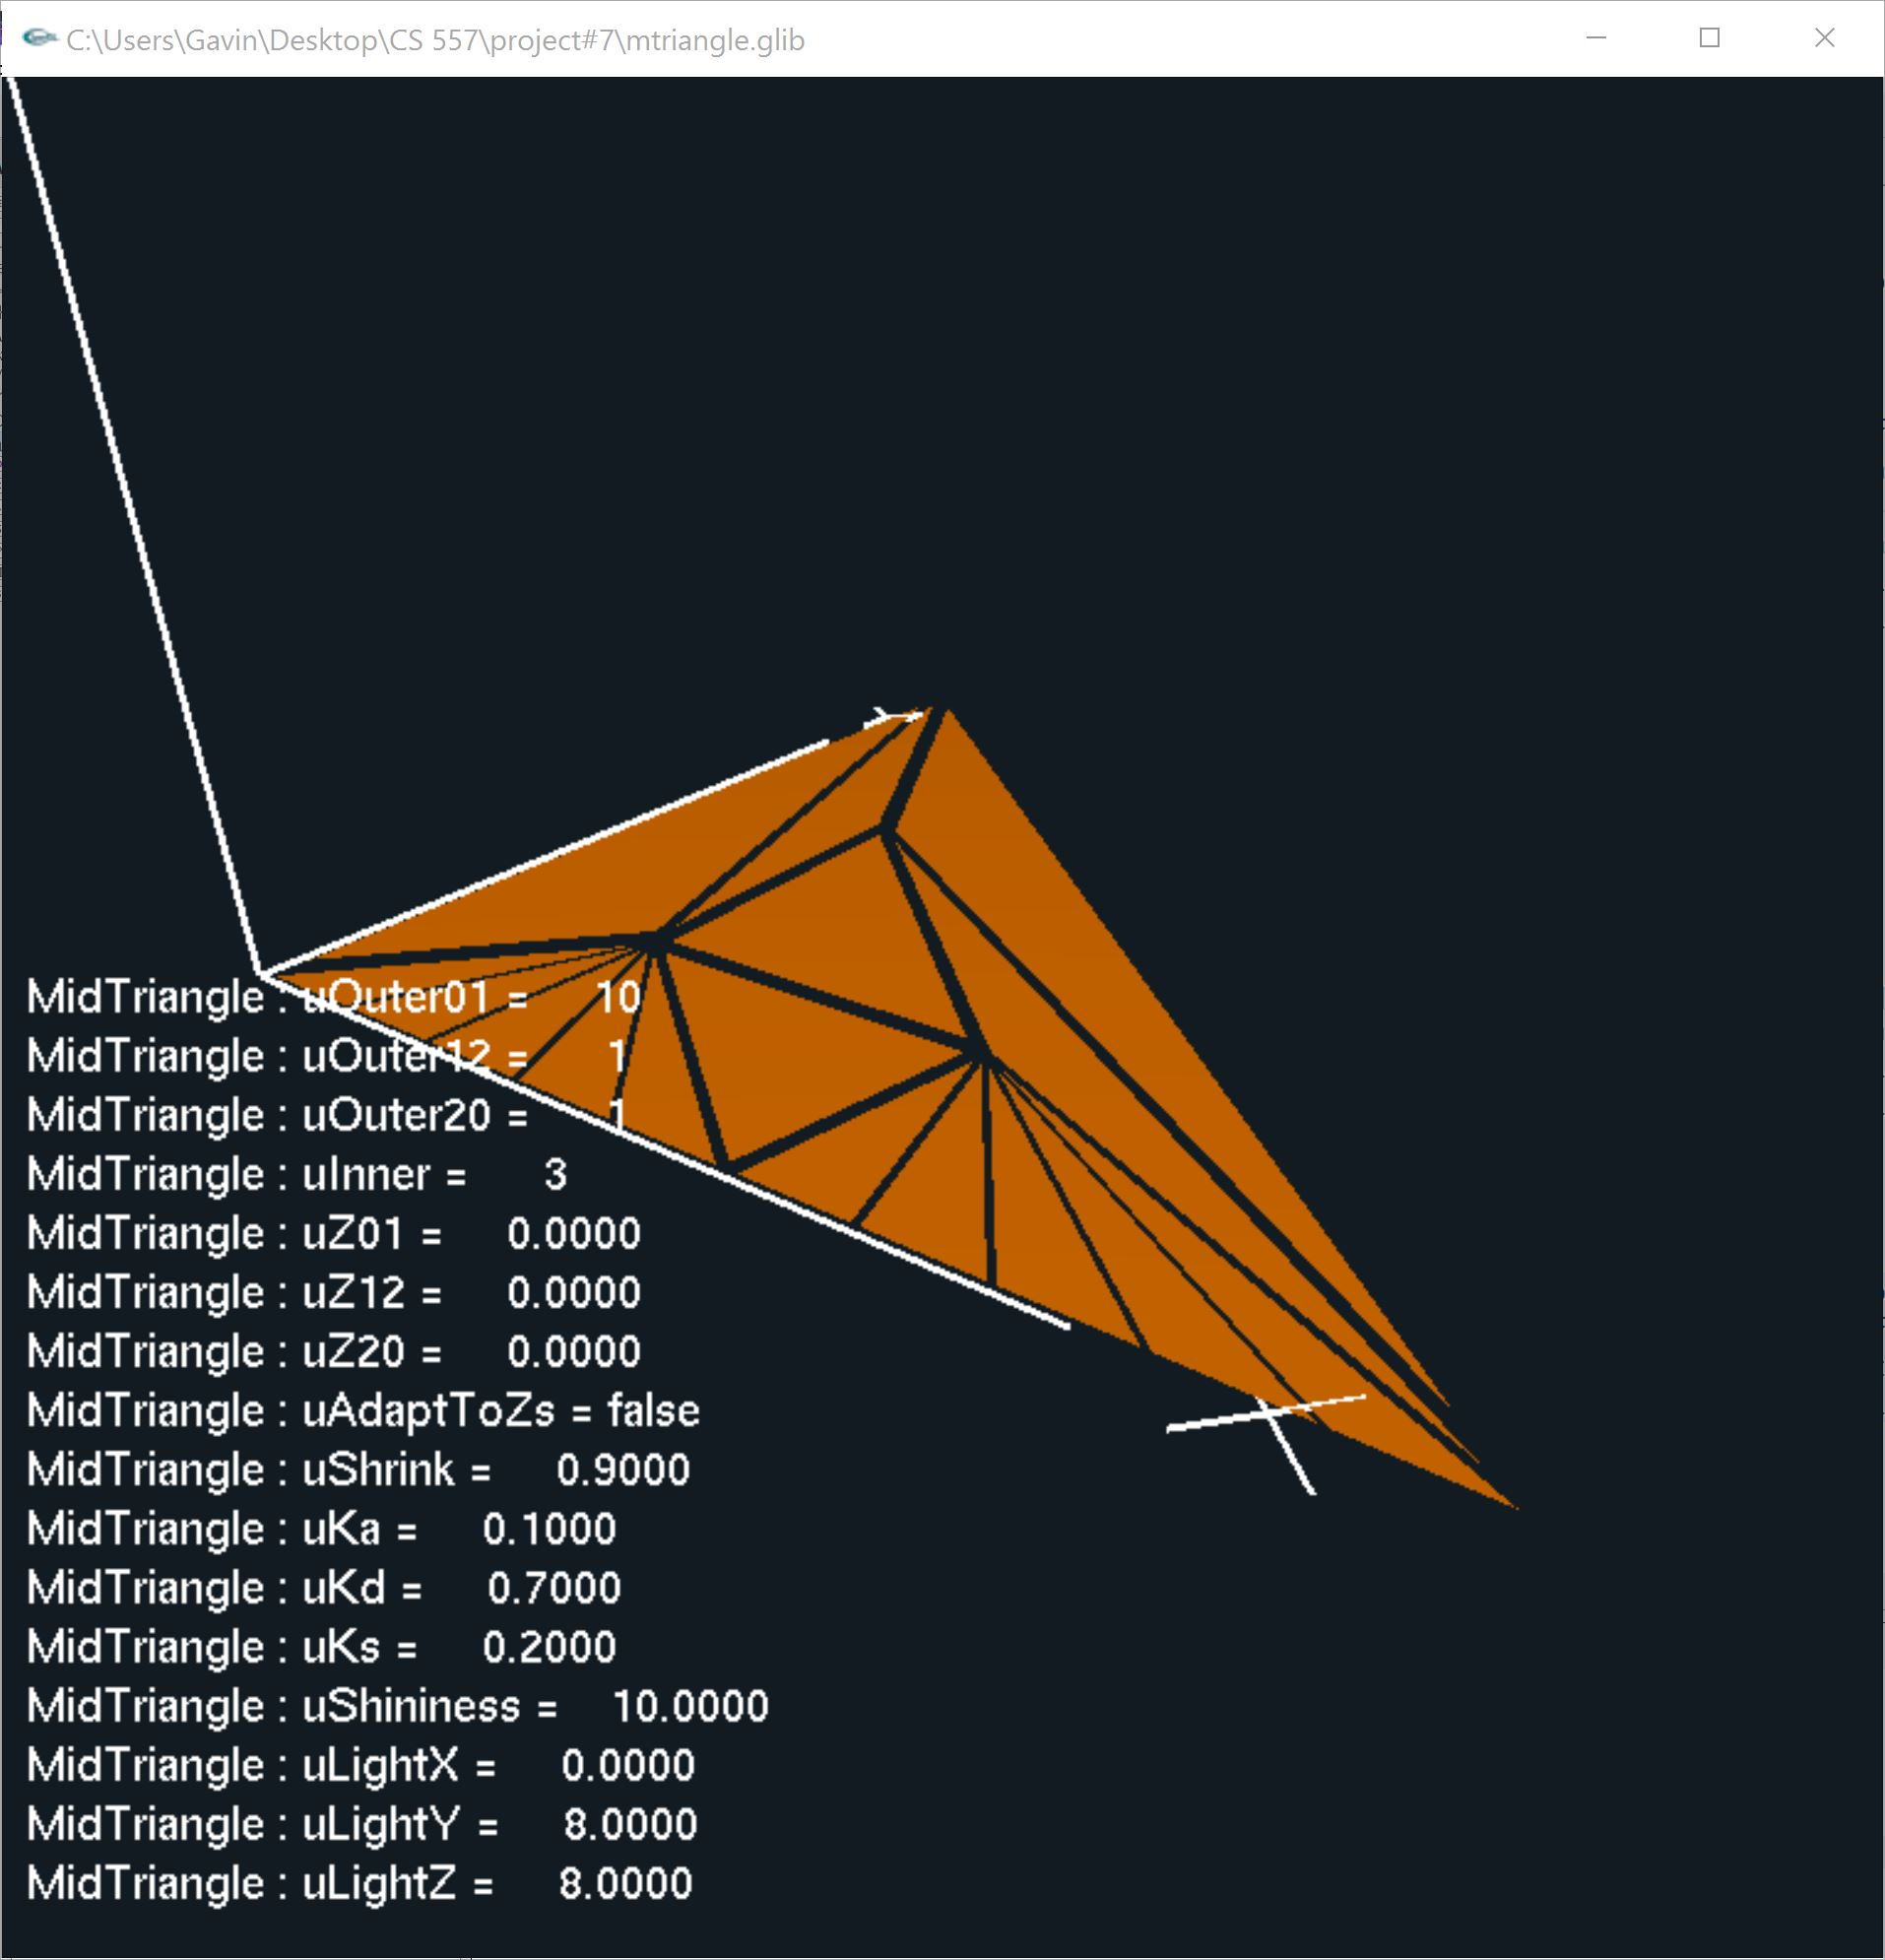
\includegraphics[width=3.2in]{out01.jpg}
	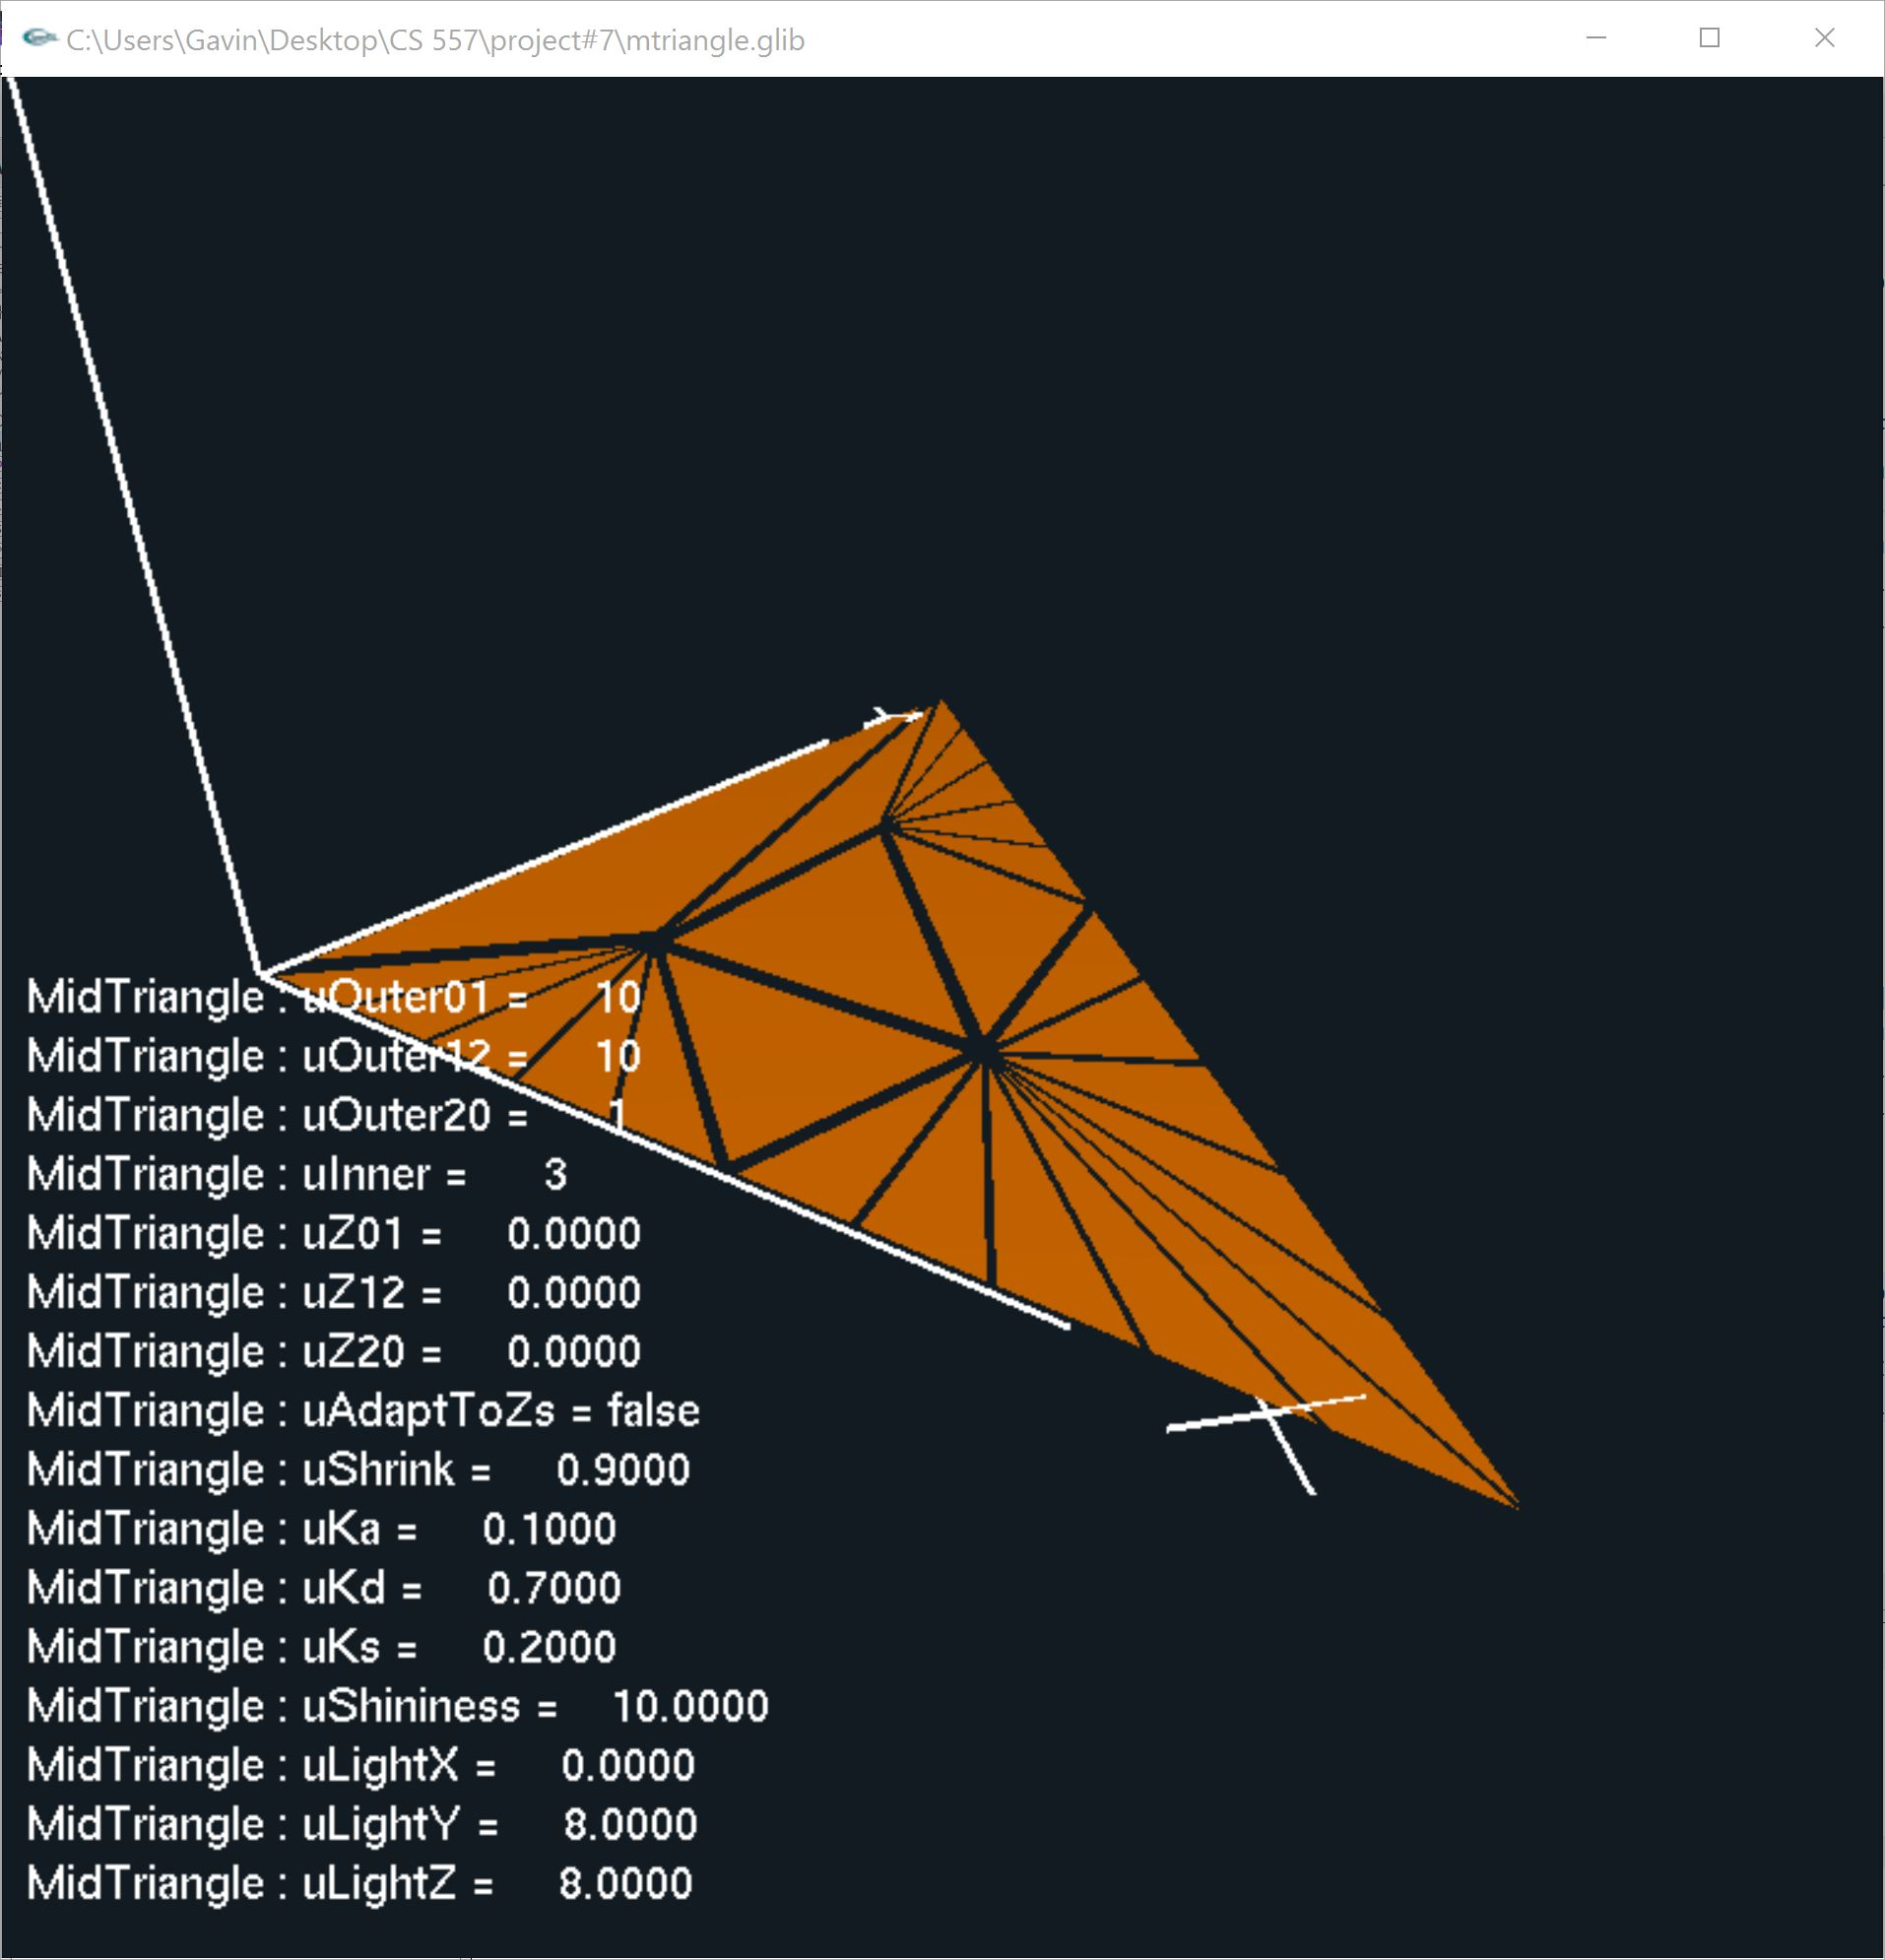
\includegraphics[width=3.2in]{out12.jpg}
	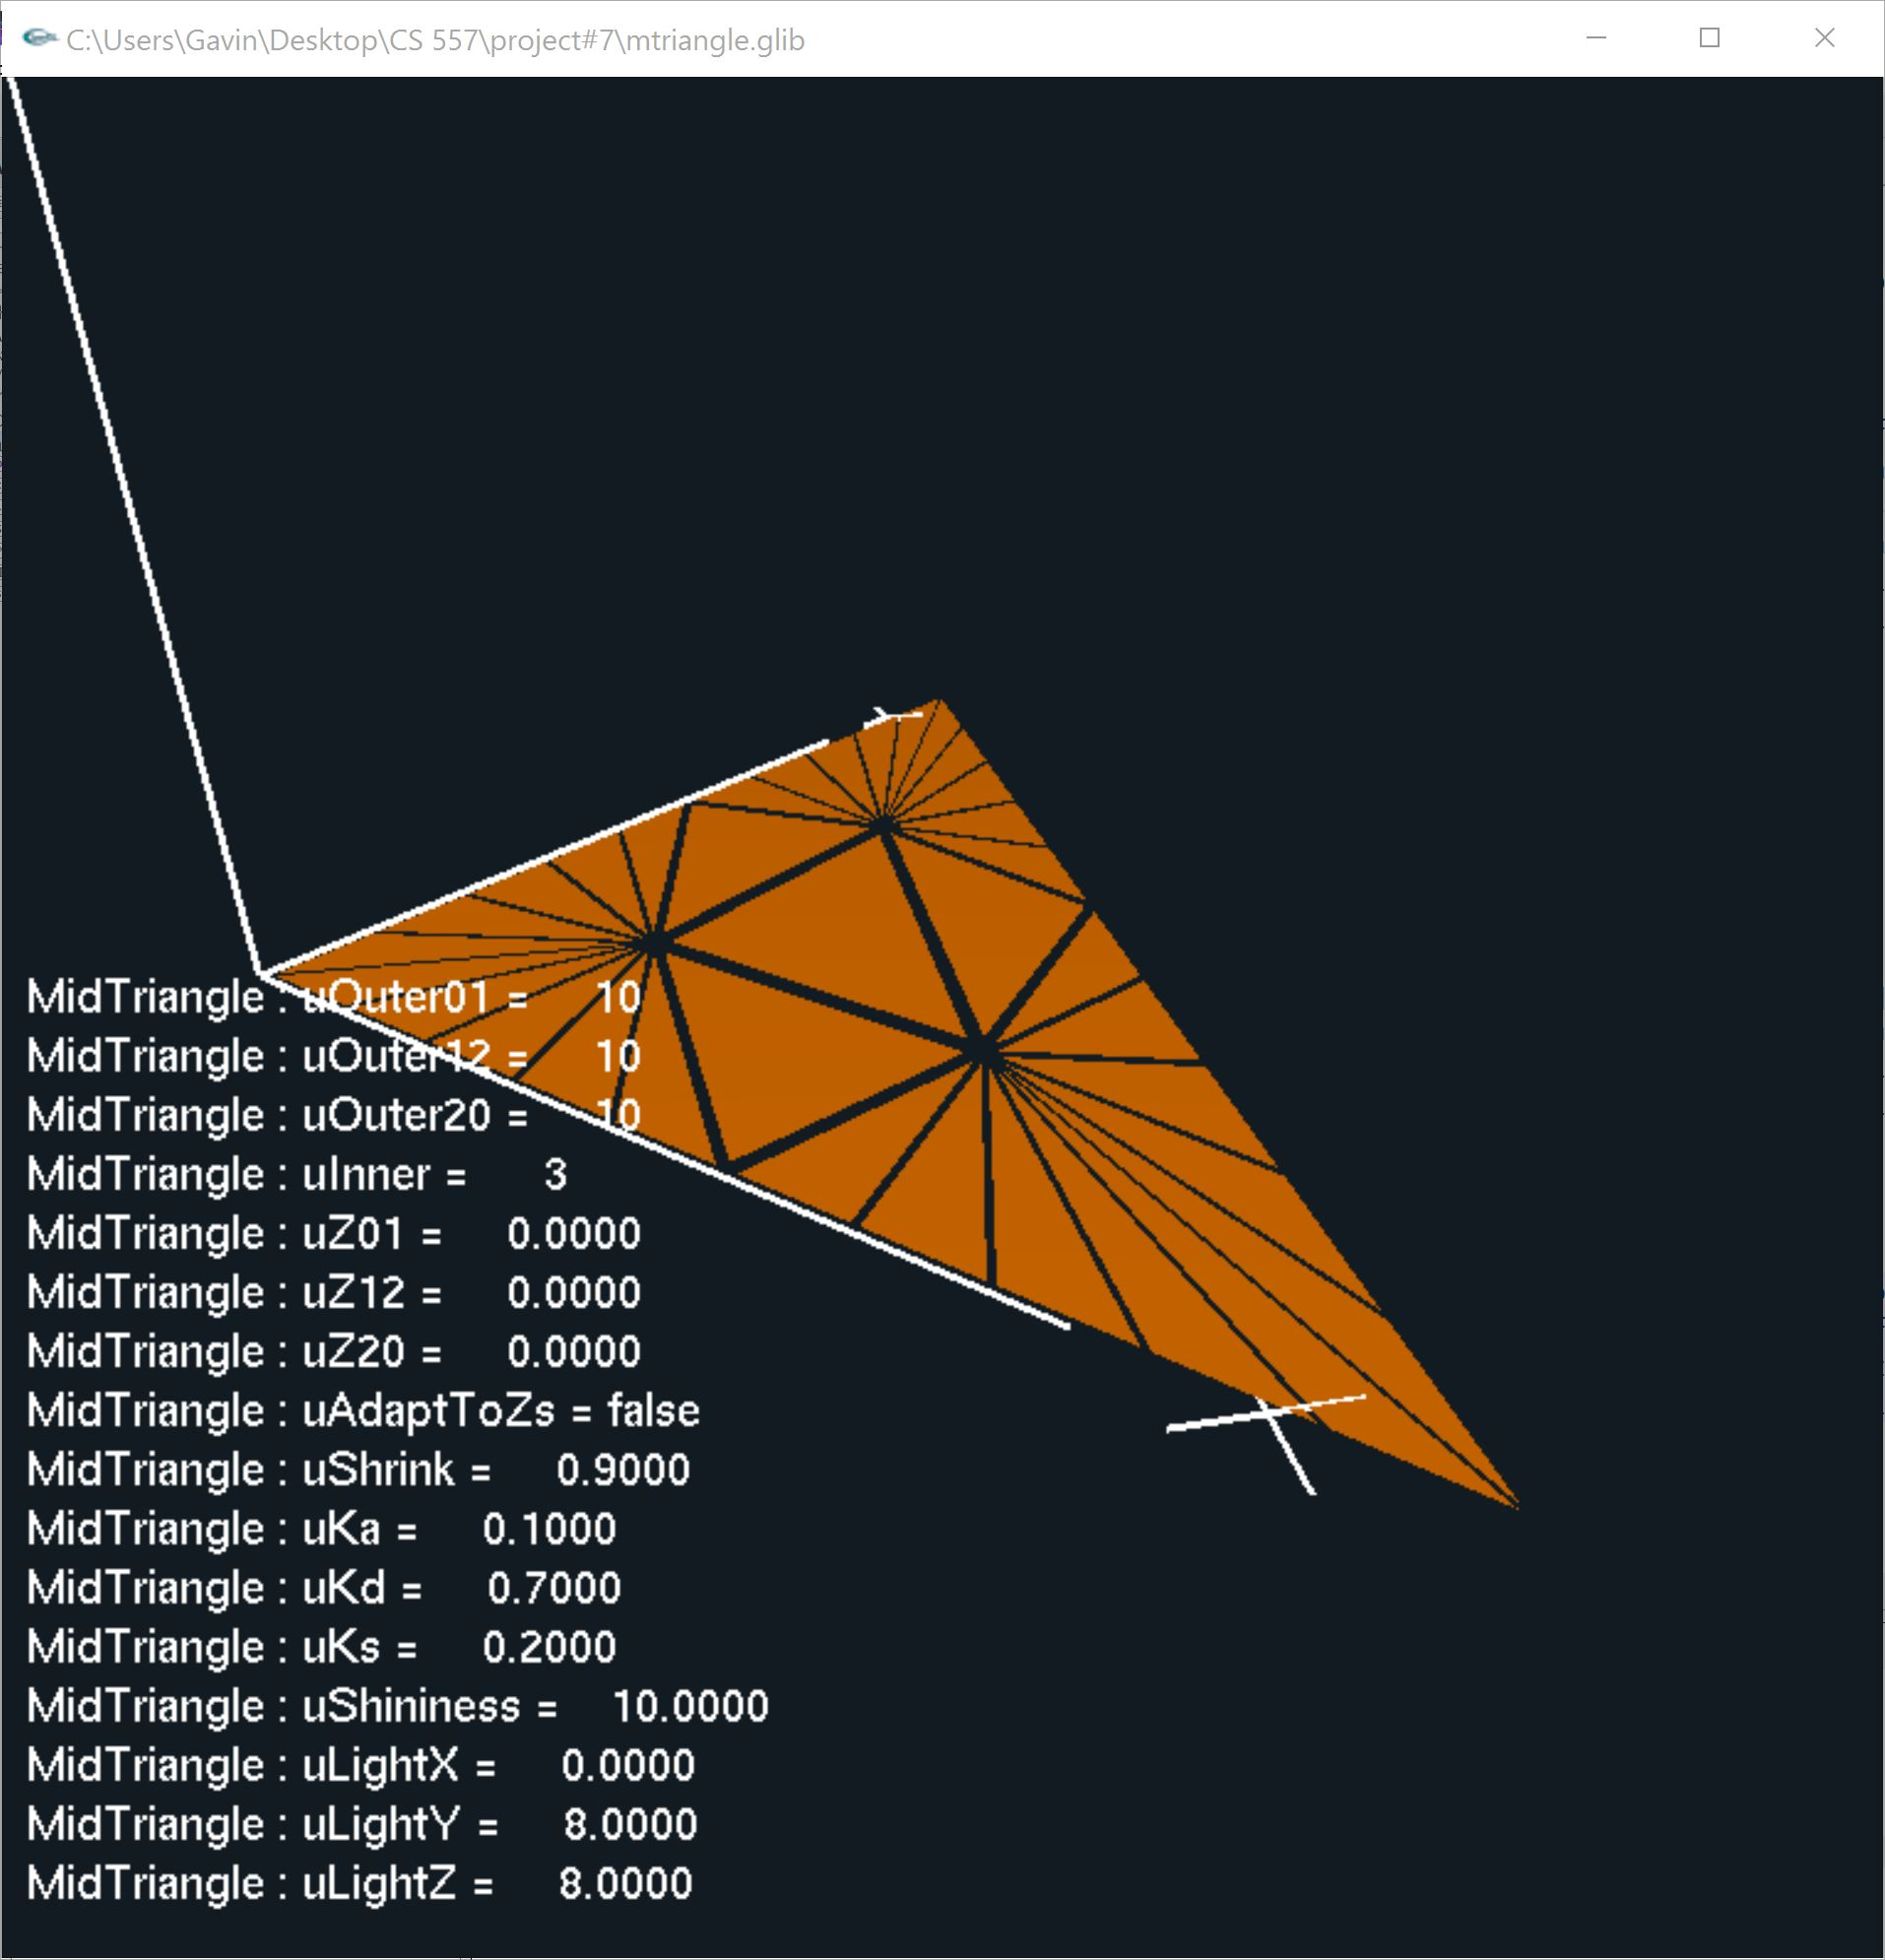
\includegraphics[width=3.2in]{out20.jpg}
	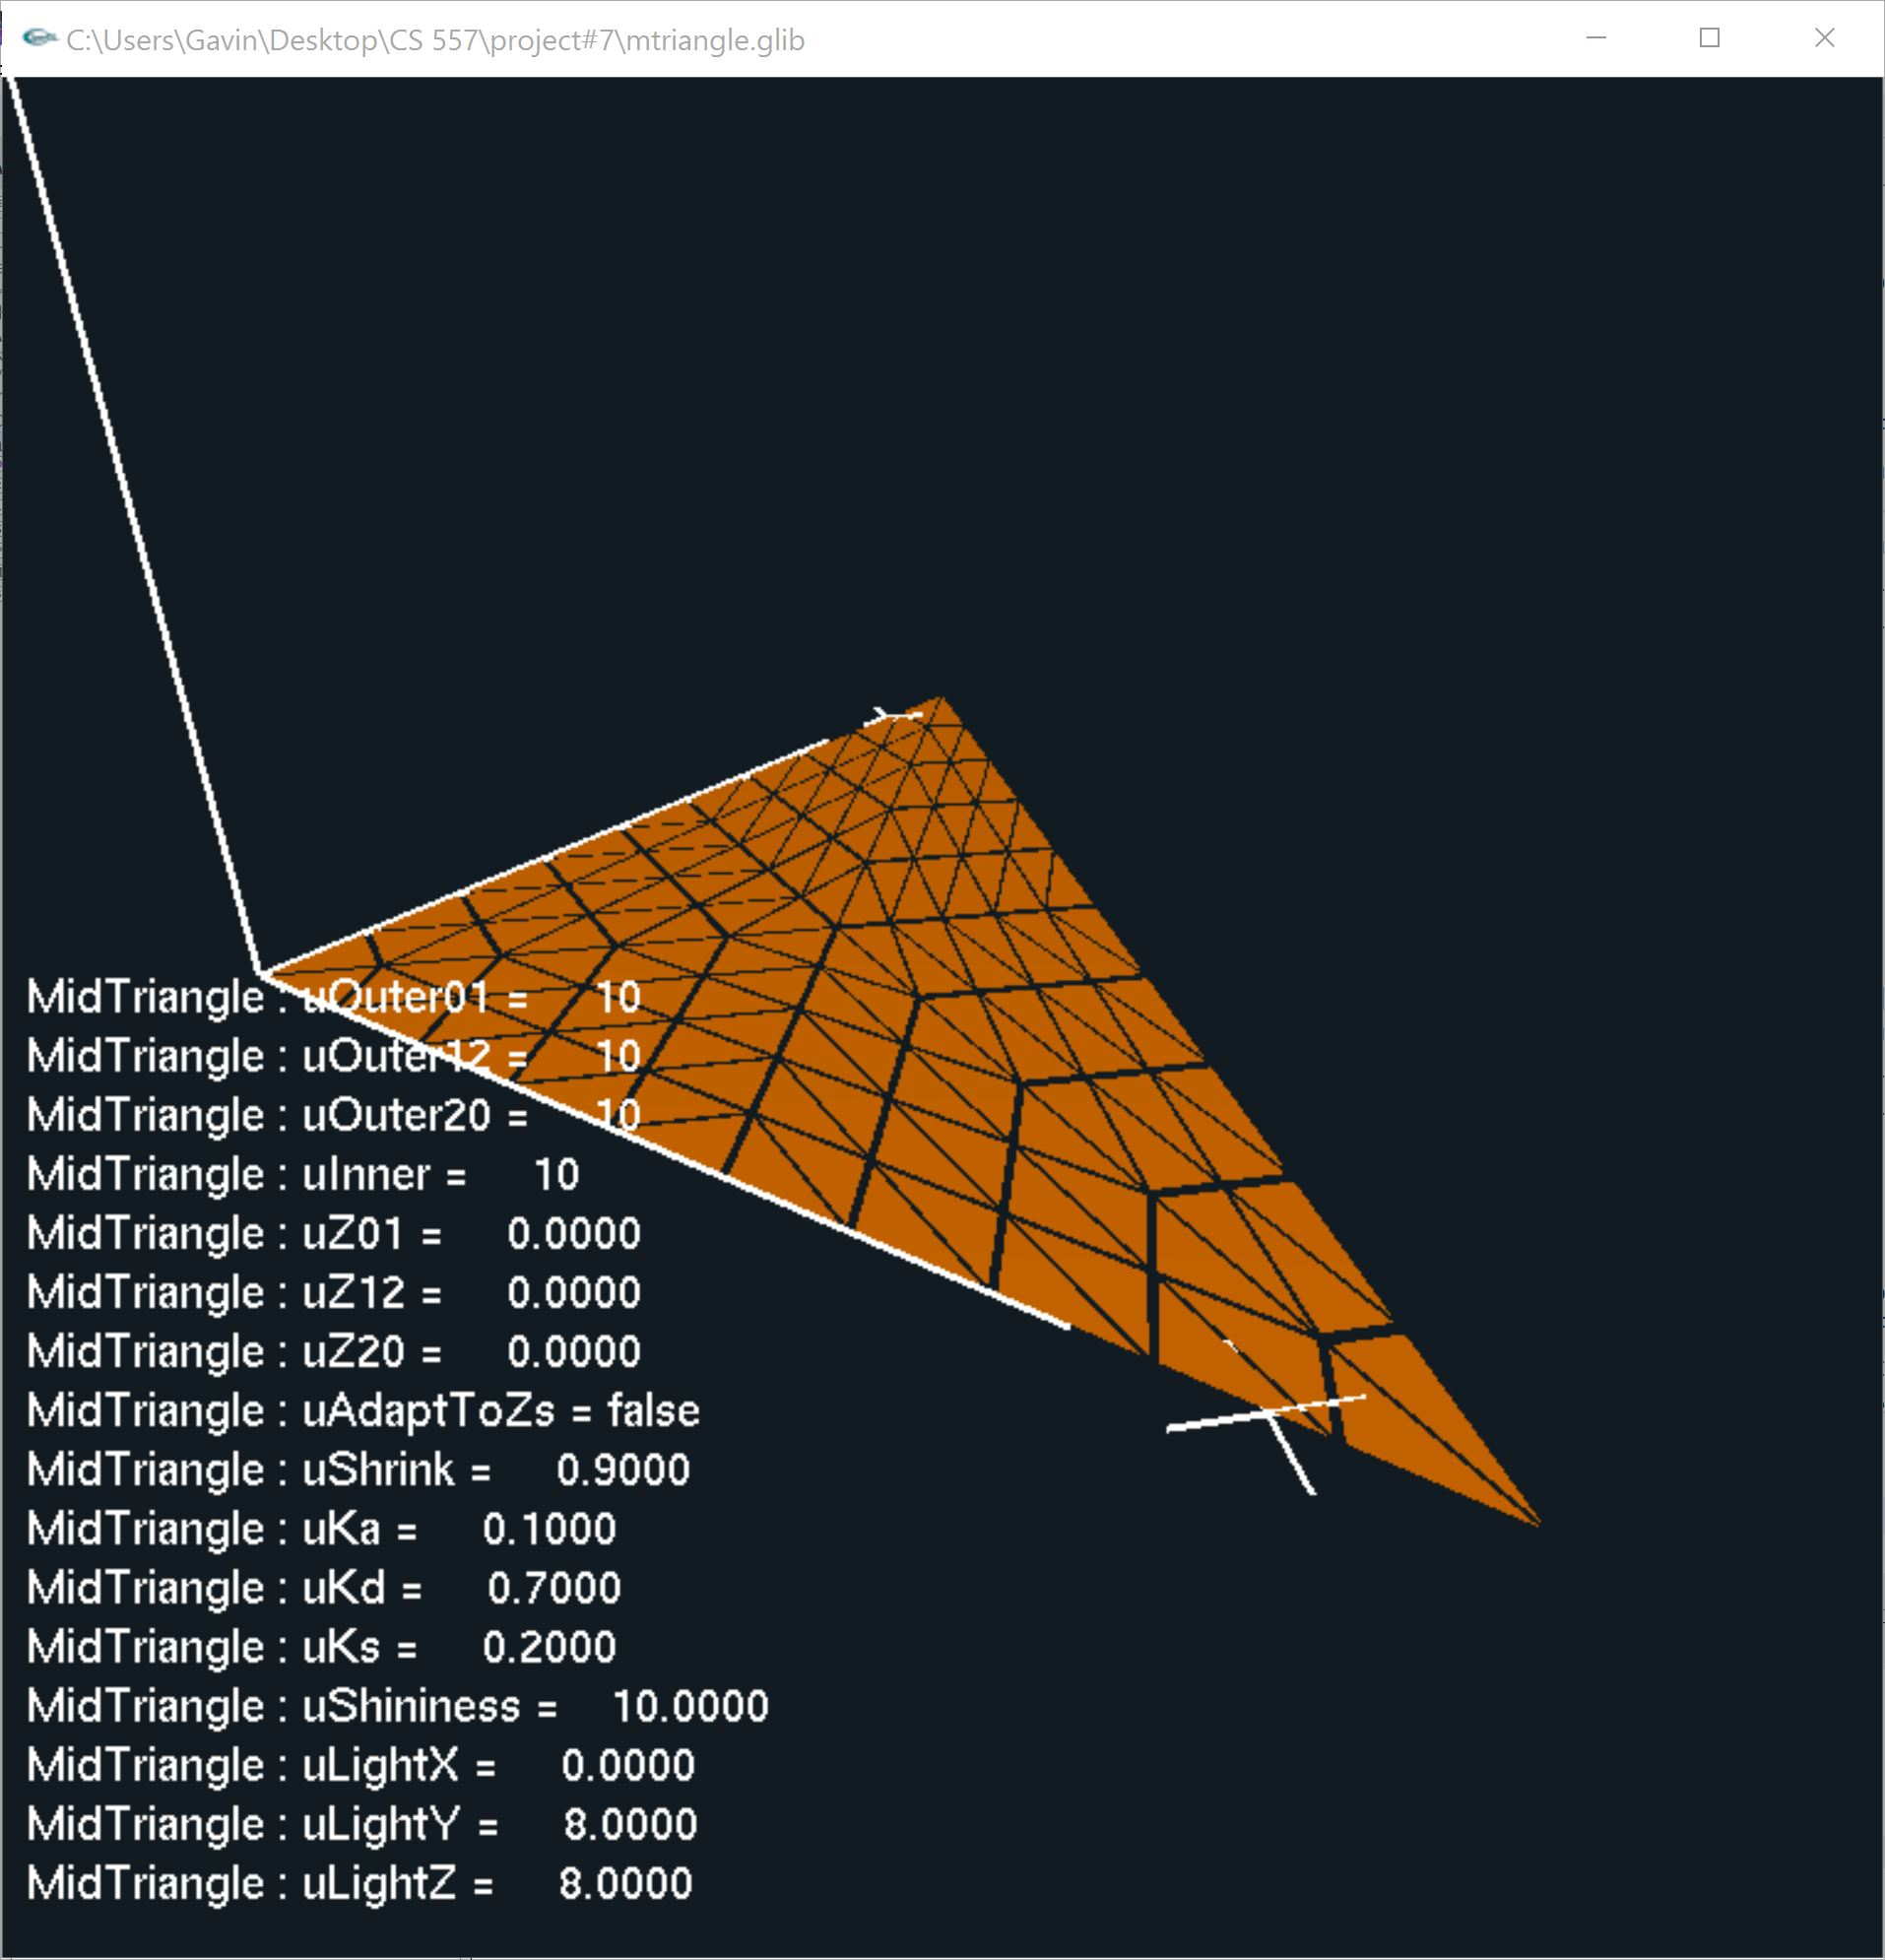
\includegraphics[width=3.2in]{inner.jpg}
\end{center}
In the previous images, the light looks like doesn't exist. However the truth is the light does exist but is not obvious from the particular angle. By changing some lighting parameters and rotating the patch for a particular angle, the light becomes easy to see. The following image shows the lighting effects.
\begin{center}
	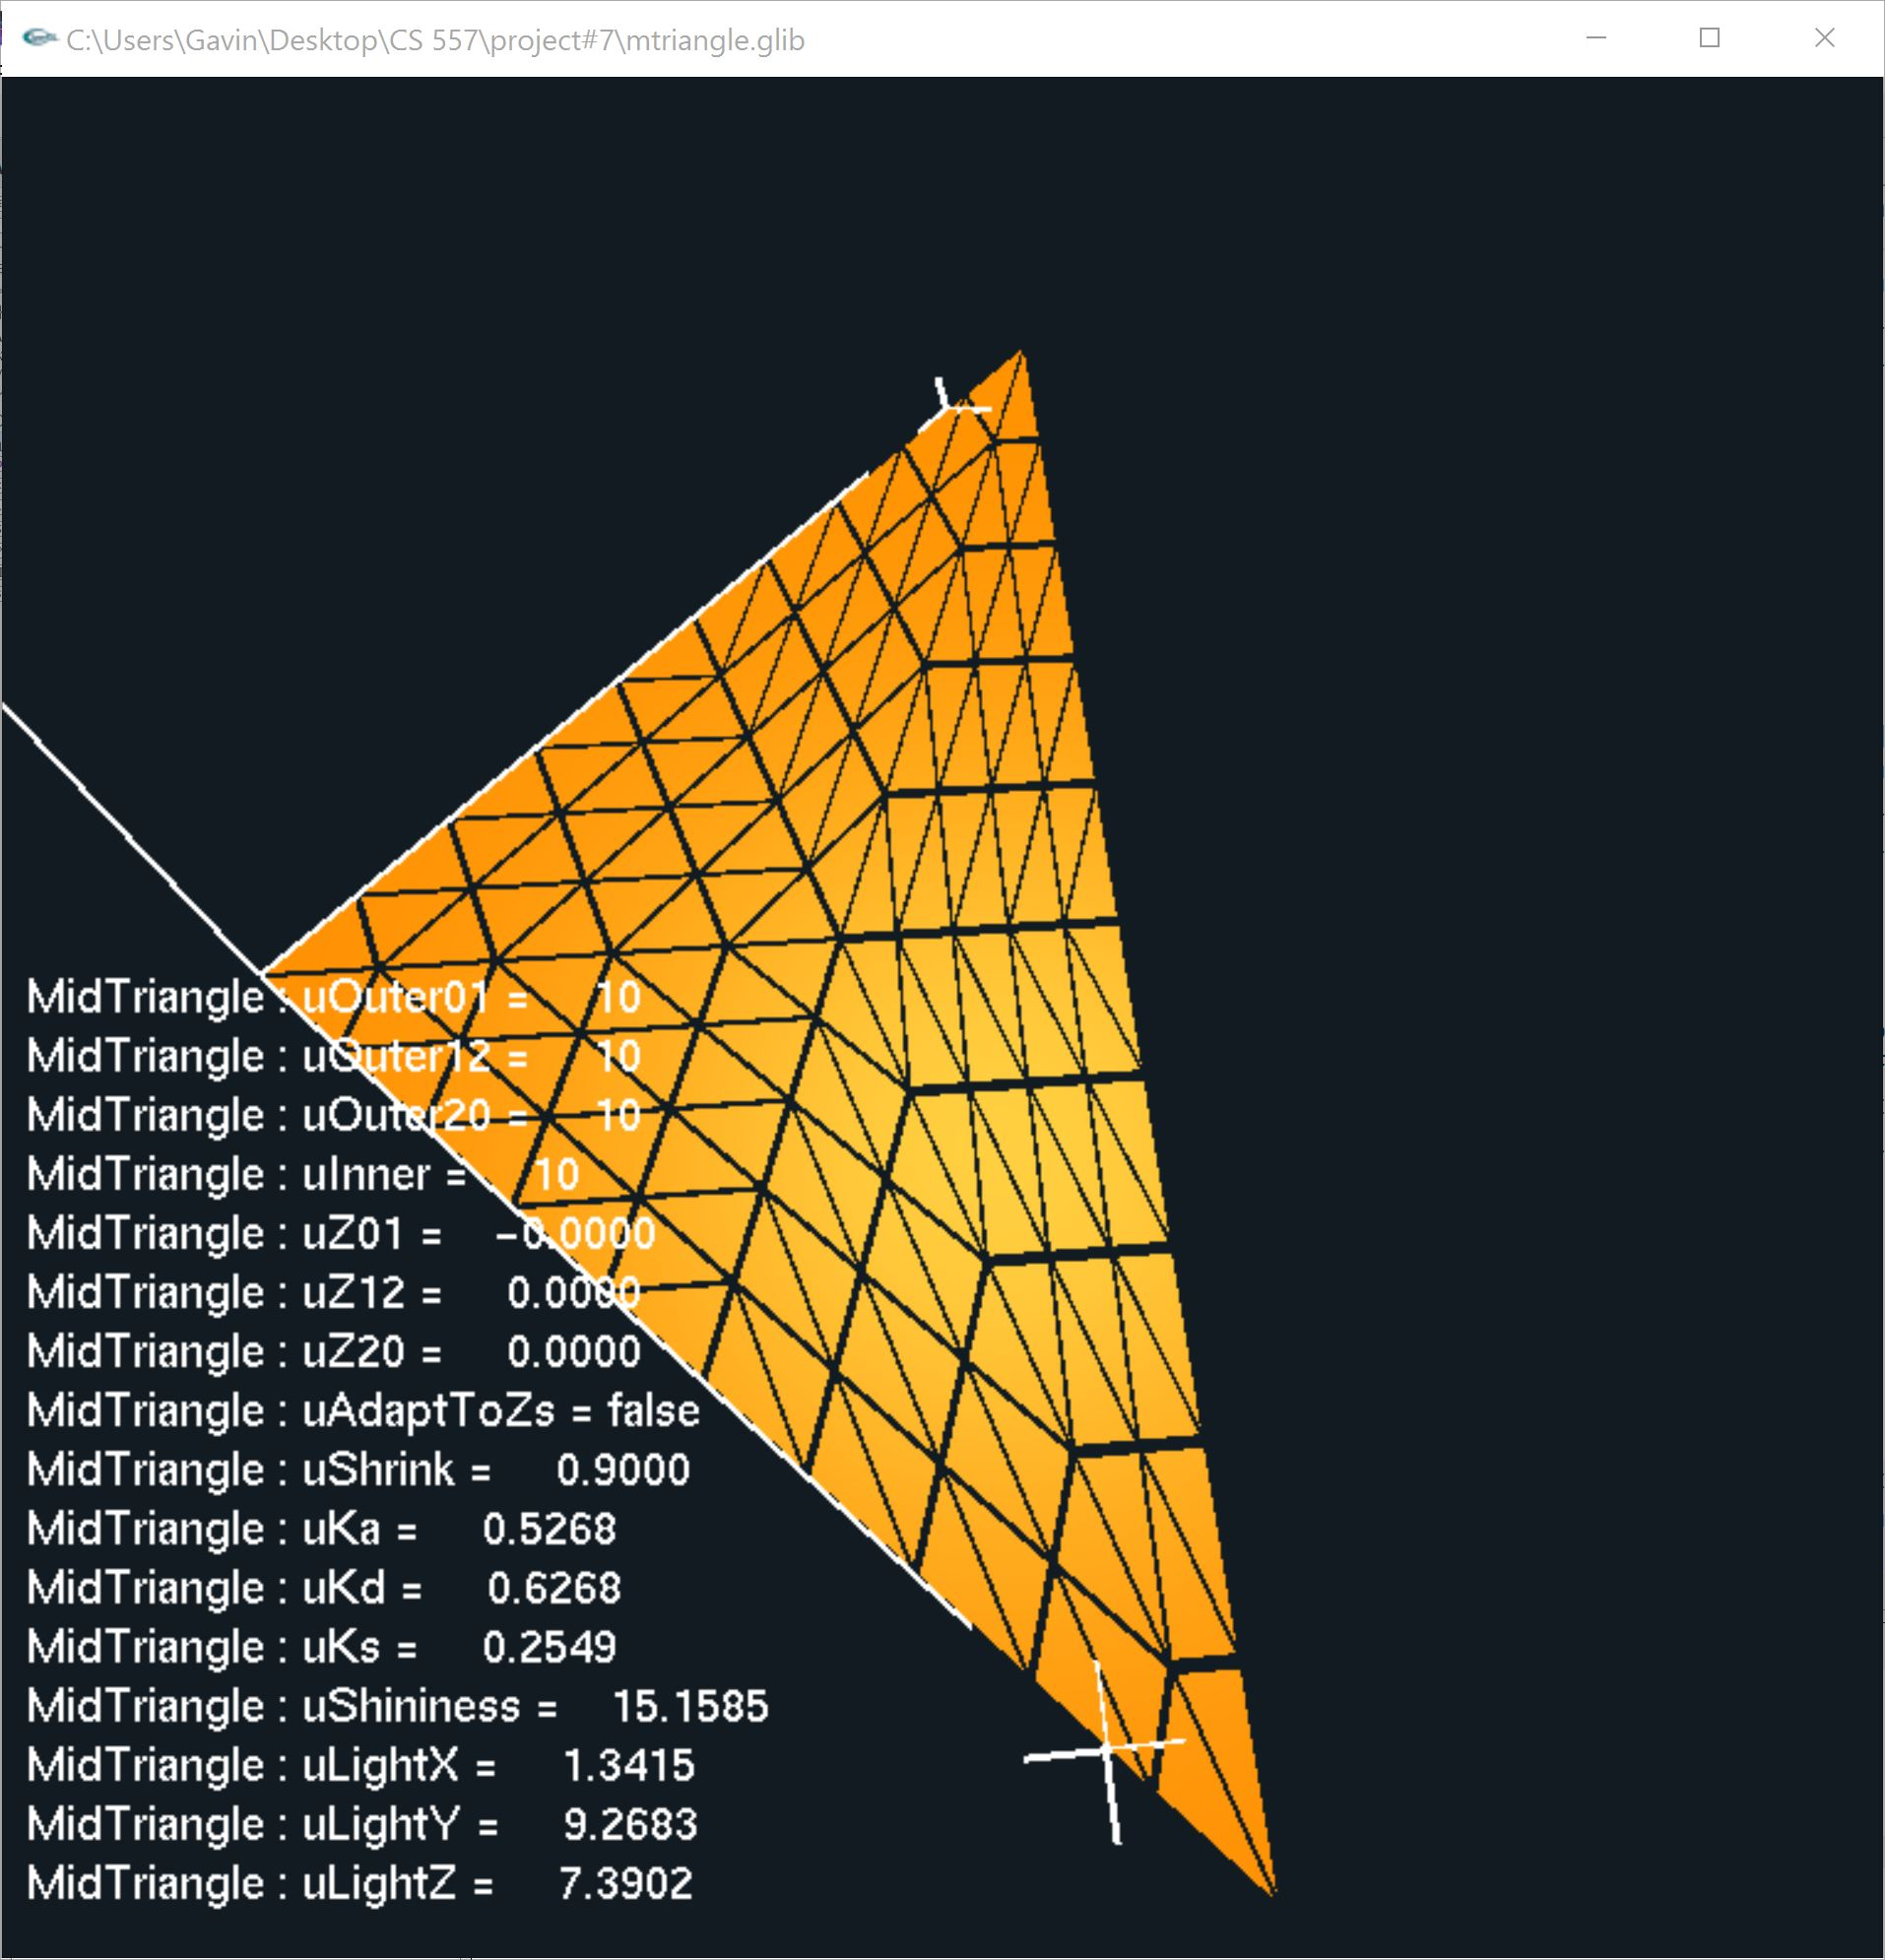
\includegraphics[width=3.2in]{light.jpg}
\end{center}
The z values of each edge's center are also controlled by sliders. Since this is a B\'{e}zier patch, only change the center point of each edge will result in a smooth curve along the edge. The following image shows the effect when the Z values are changed. The inner and outer densities are all remain in 10.
\begin{center}
	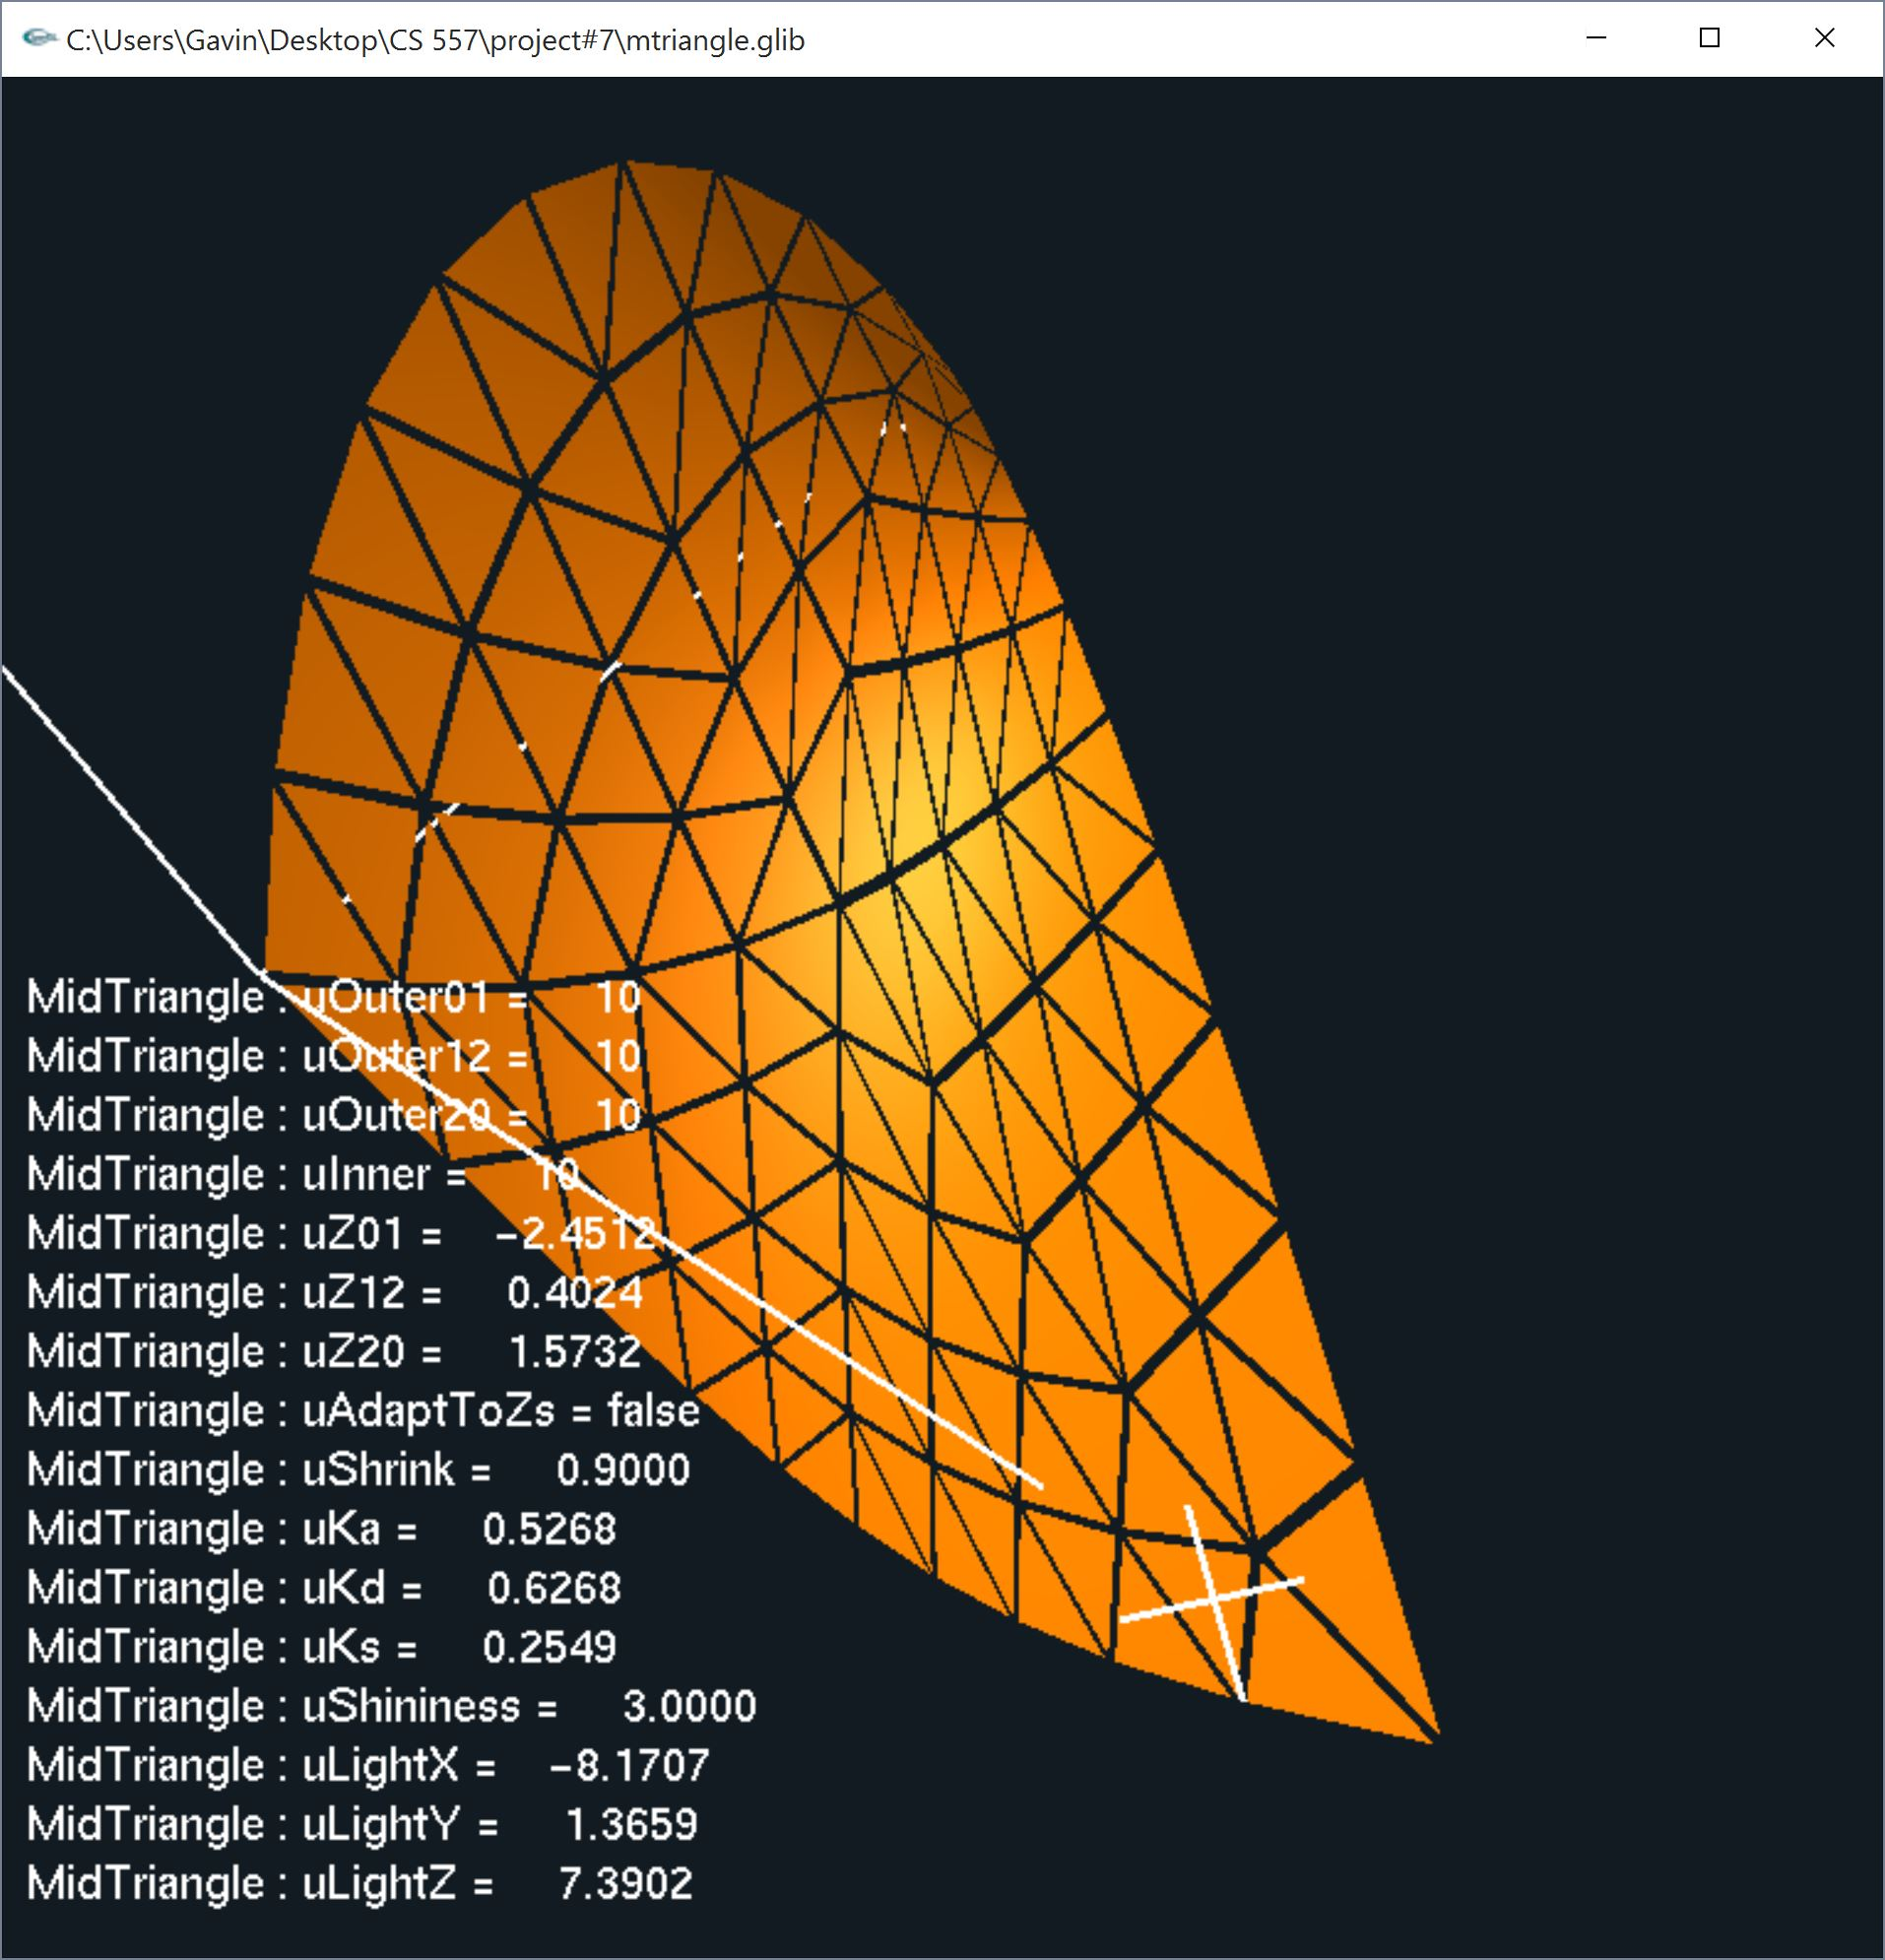
\includegraphics[width=3.2in]{changeZ.jpg}
\end{center}
There exists a checkbox named ``uAdaptToZs''. When the checkbox is selected, the inner and outer densities are no longer controlled by sliders but controlled by the Z values in the model coordinate. The more the vertexes away from X-Y plane, the more densities the edge has. This is set to implement a smooth edge and surface. The equation used for implementing the effect is: \textbf{gl\_TessLevelOuter=float(20*(abs(uZ)+0.5))}. The following images shows the difference that the checkbox is selected or not. The one on the left has the checkbox not selected, and it has an edge not the smooth. The one on the right has the checkbox selected, and it performs a really smooth edge.
\begin{center}
	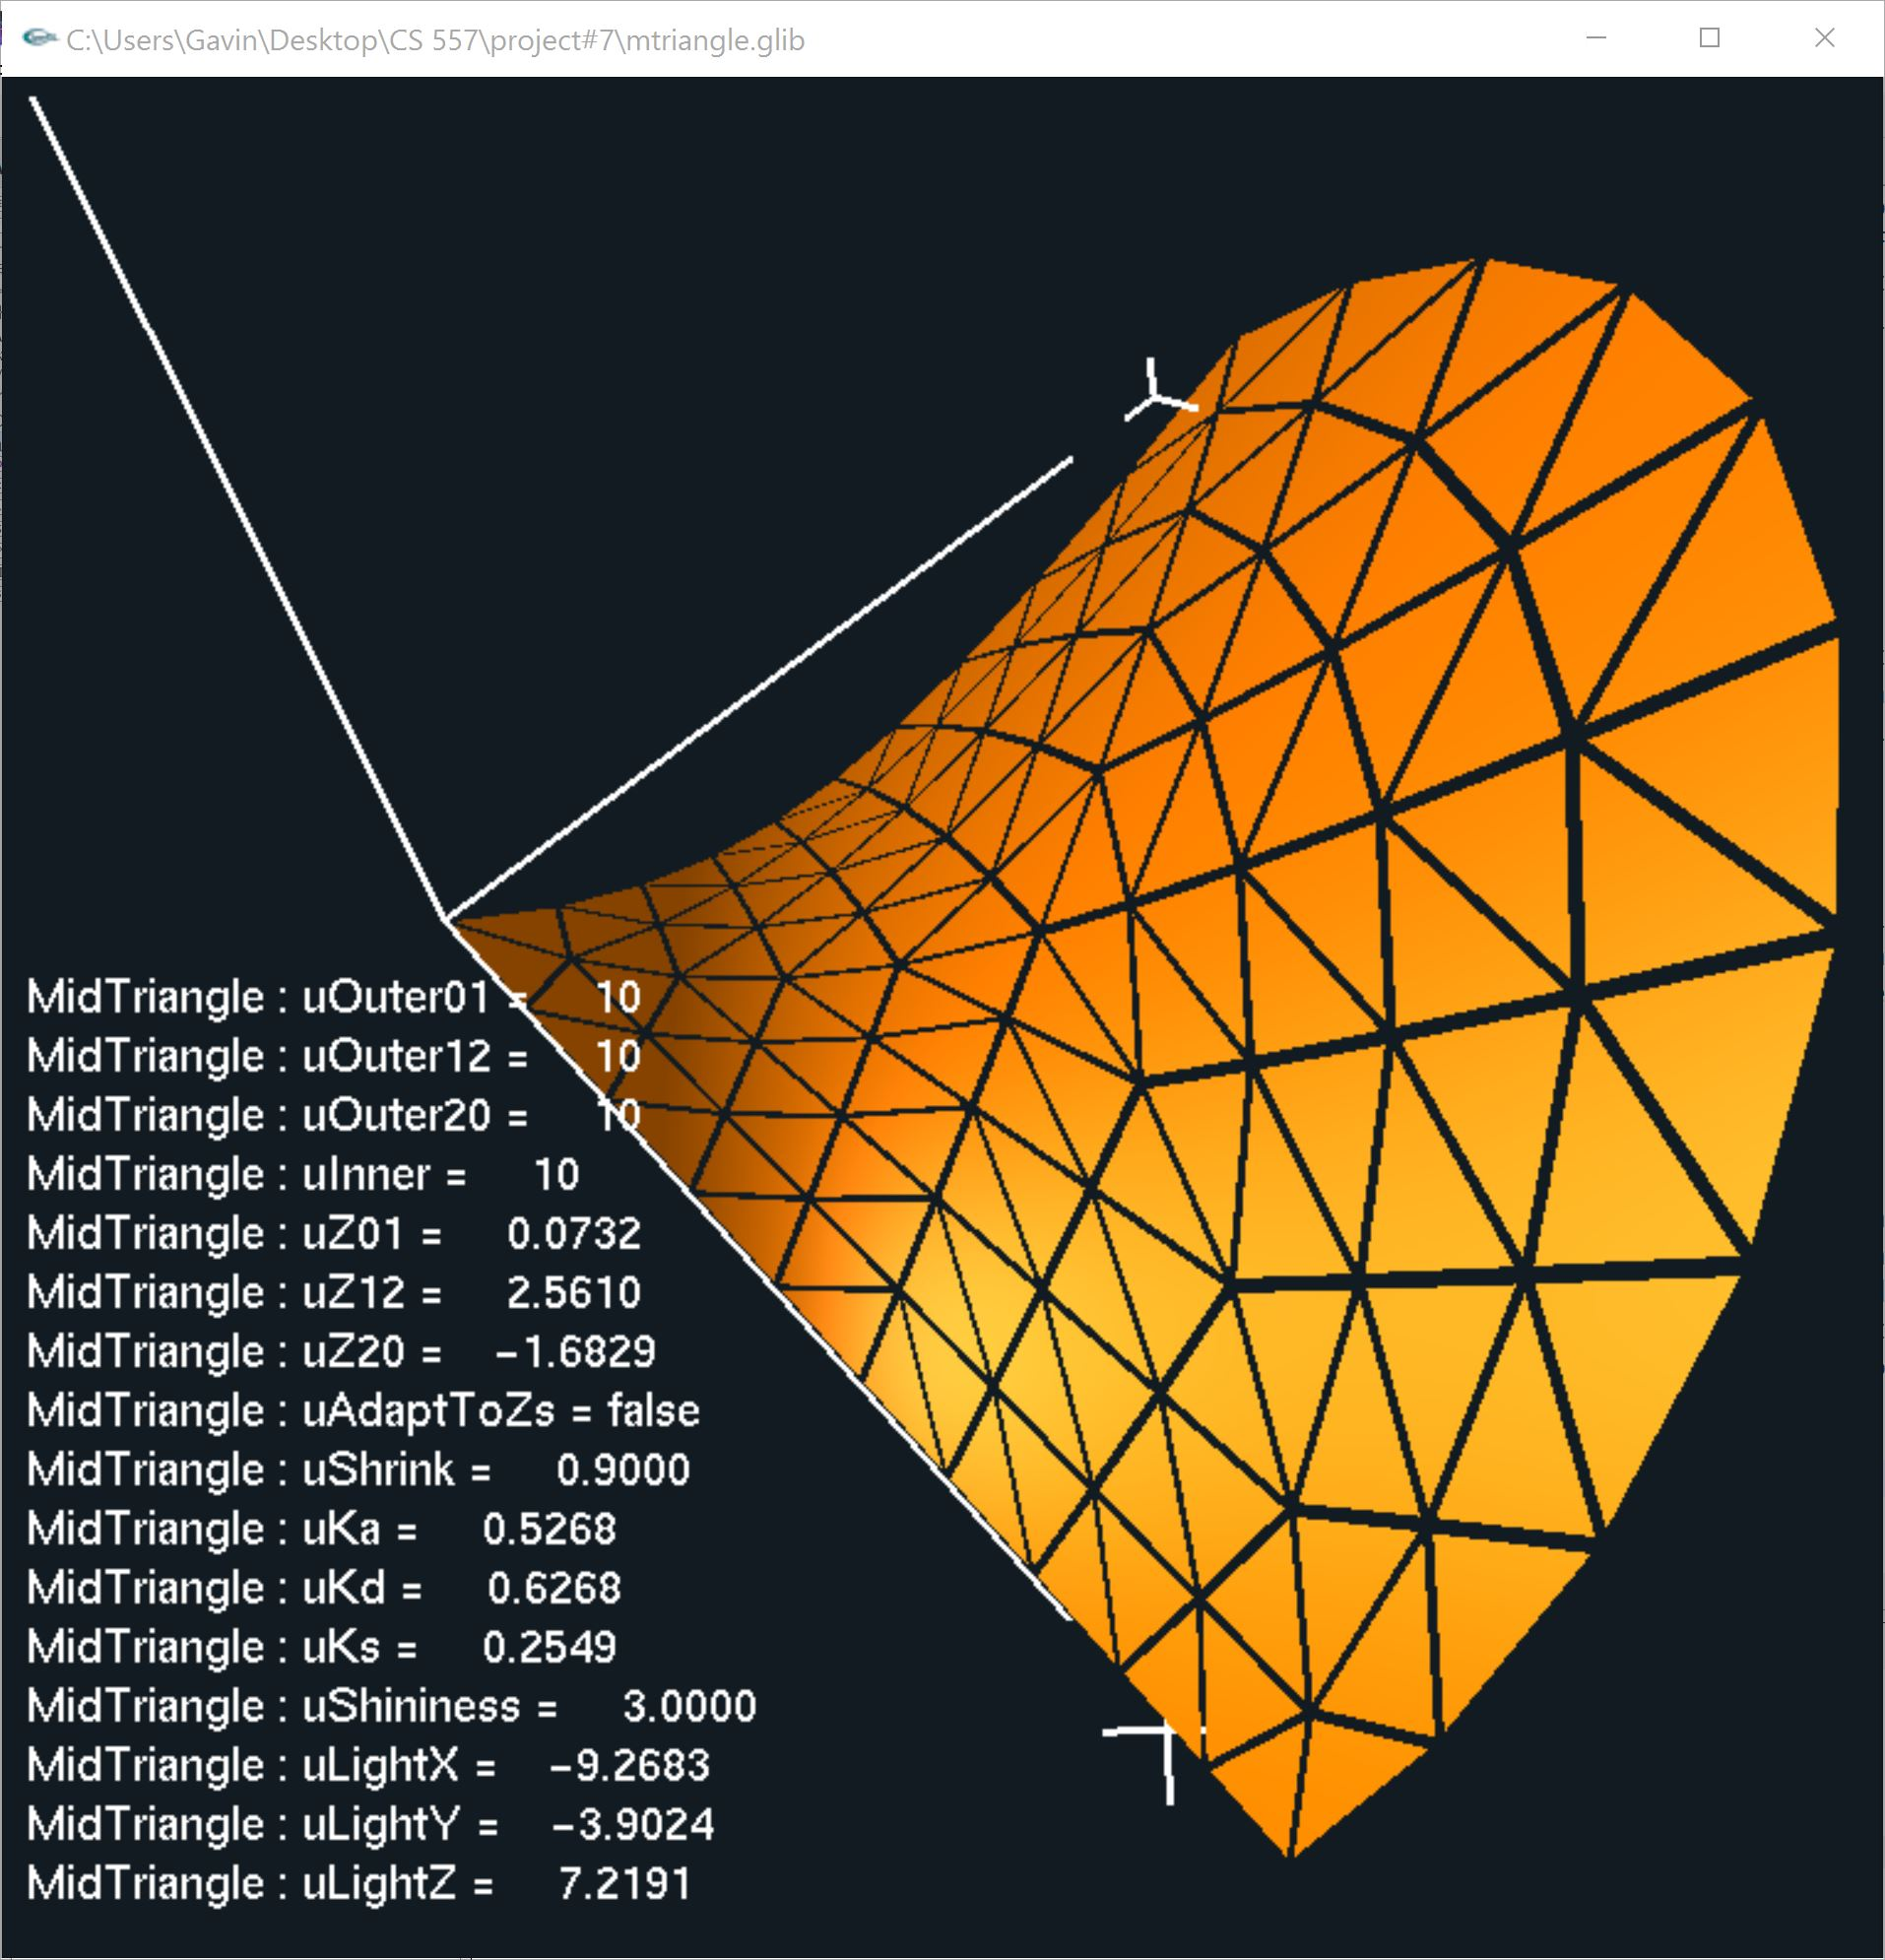
\includegraphics[width=3.2in]{adaptZ1.jpg}
	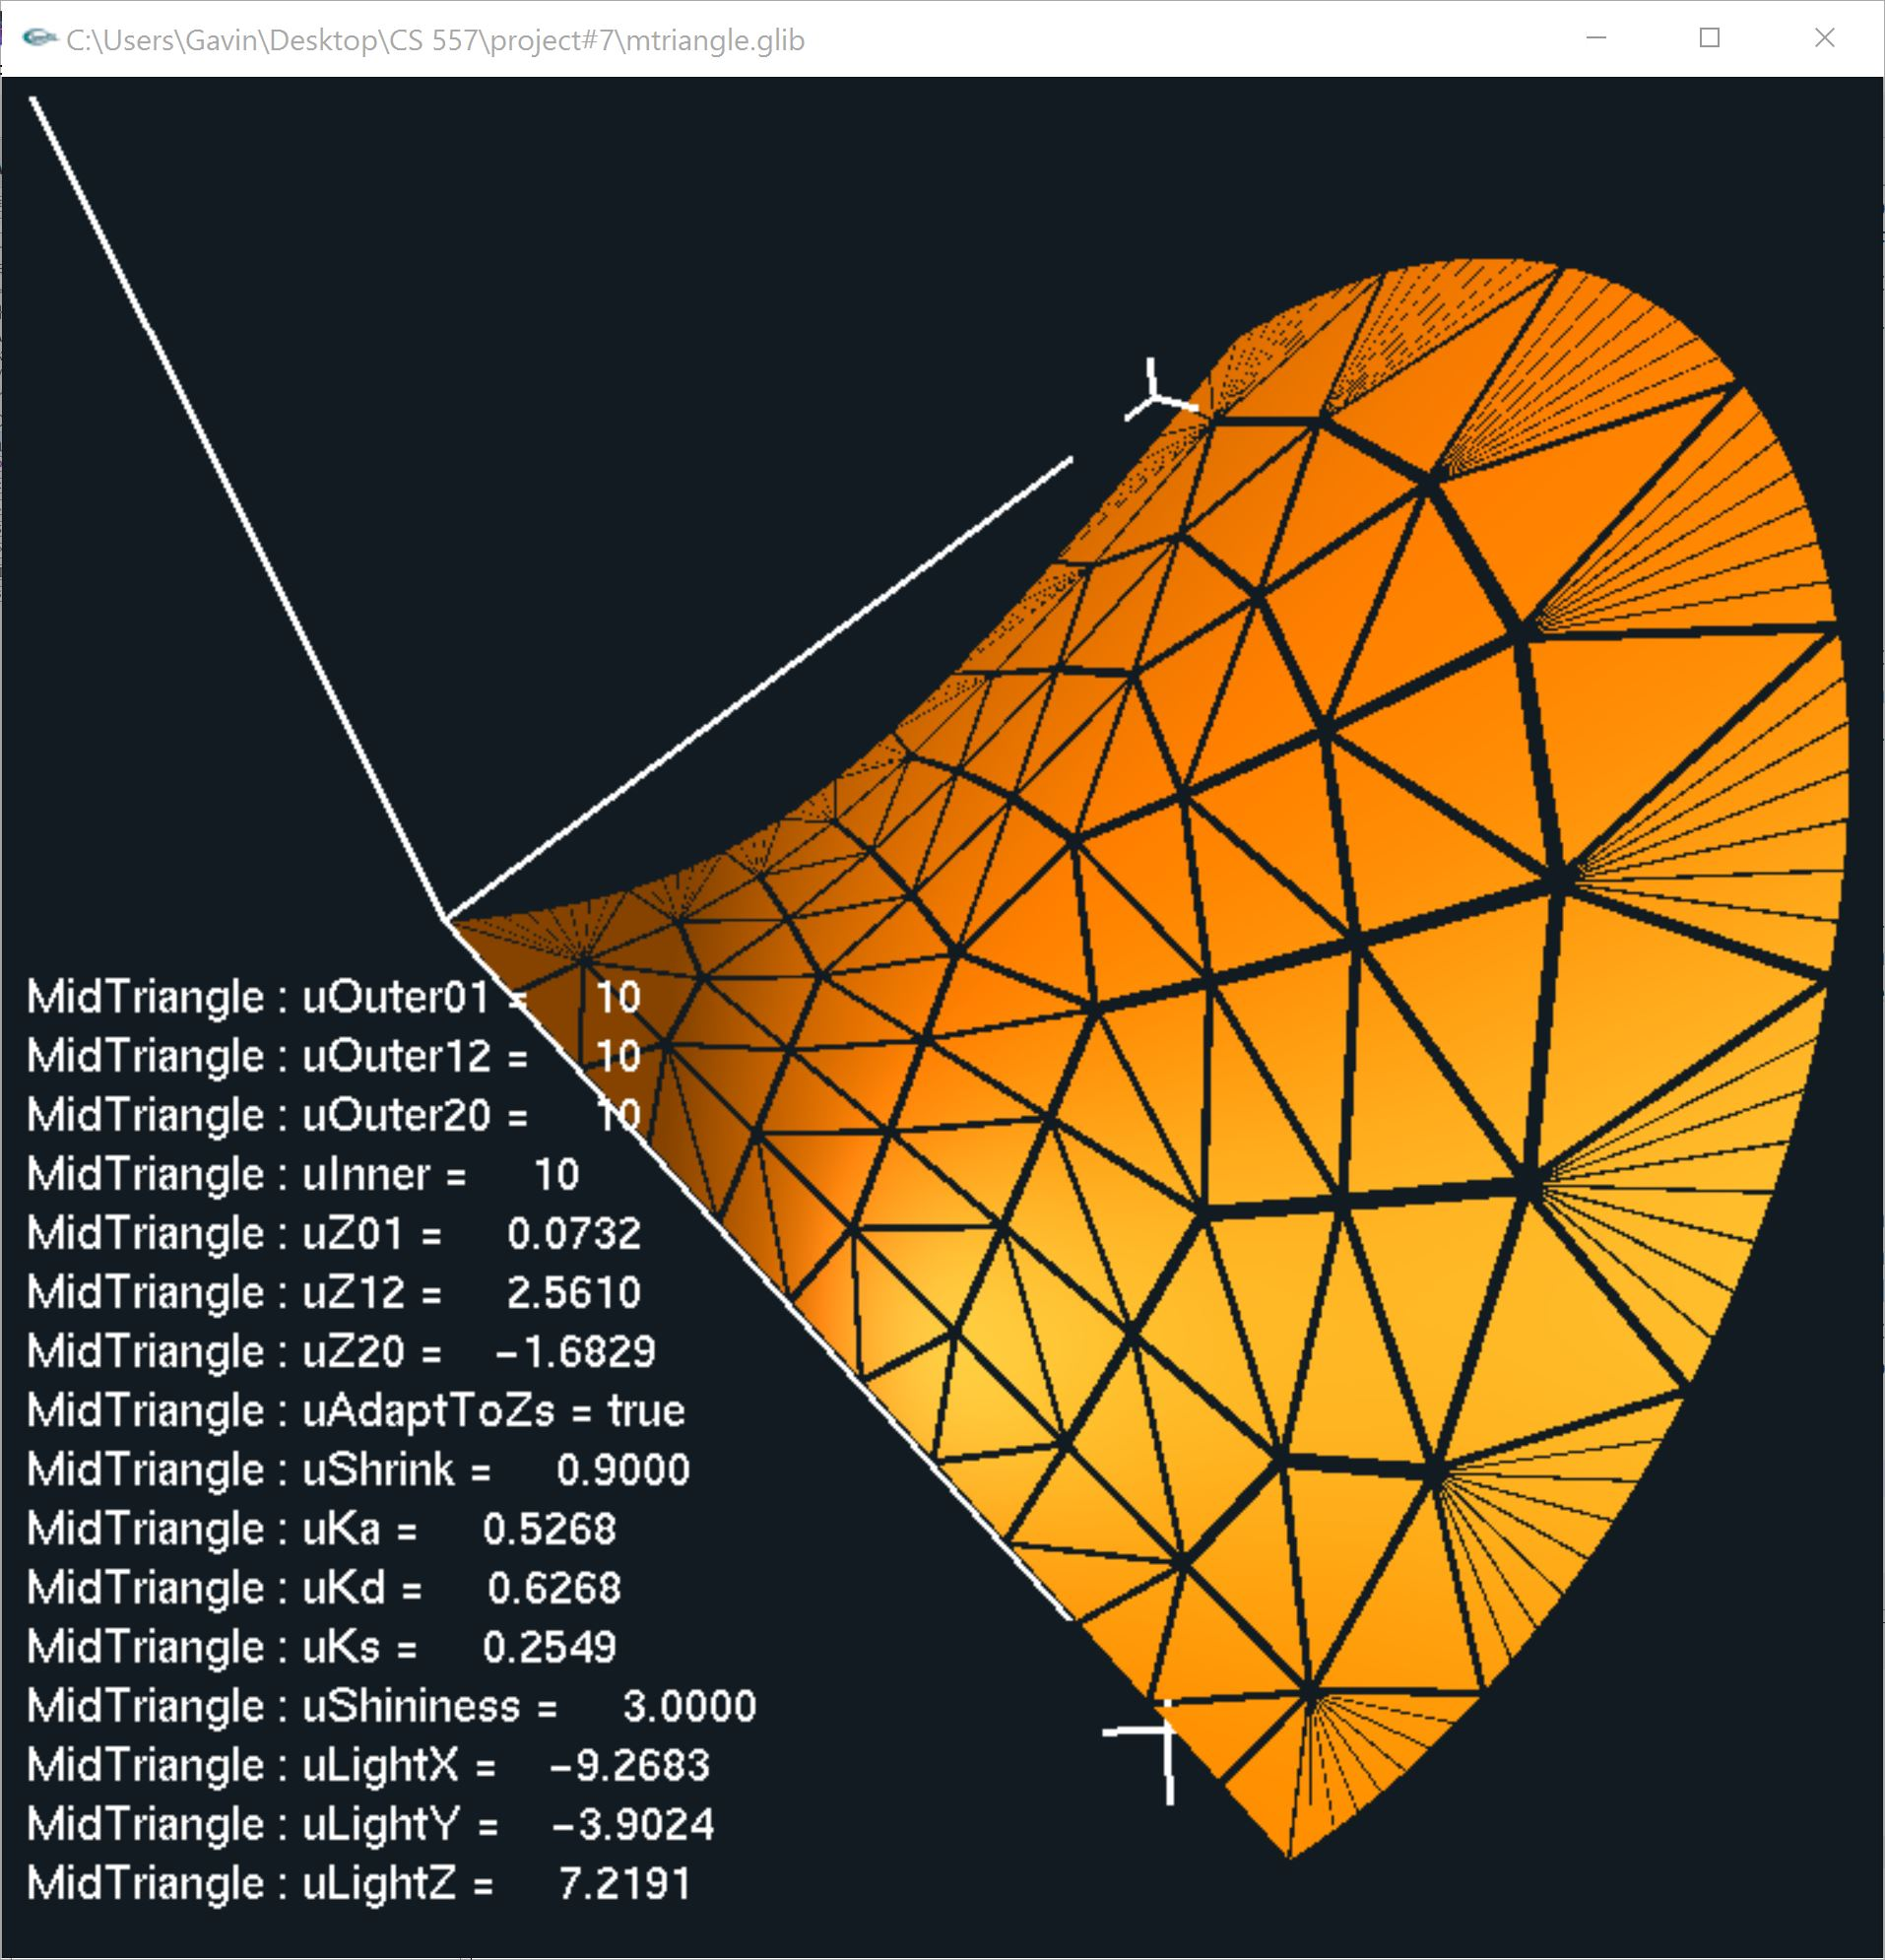
\includegraphics[width=3.2in]{adaptZ2.jpg}
\end{center}
The last feature is ``shrink''. It's controlled by geometry shader. The parameter is controlled by a slider named ``uShrink''. This slider will change the size of the triangles. When the slider has the value of 1, the whole patch will look like a solid surface. The following images show the differences when the slider is changed.
\begin{center}
	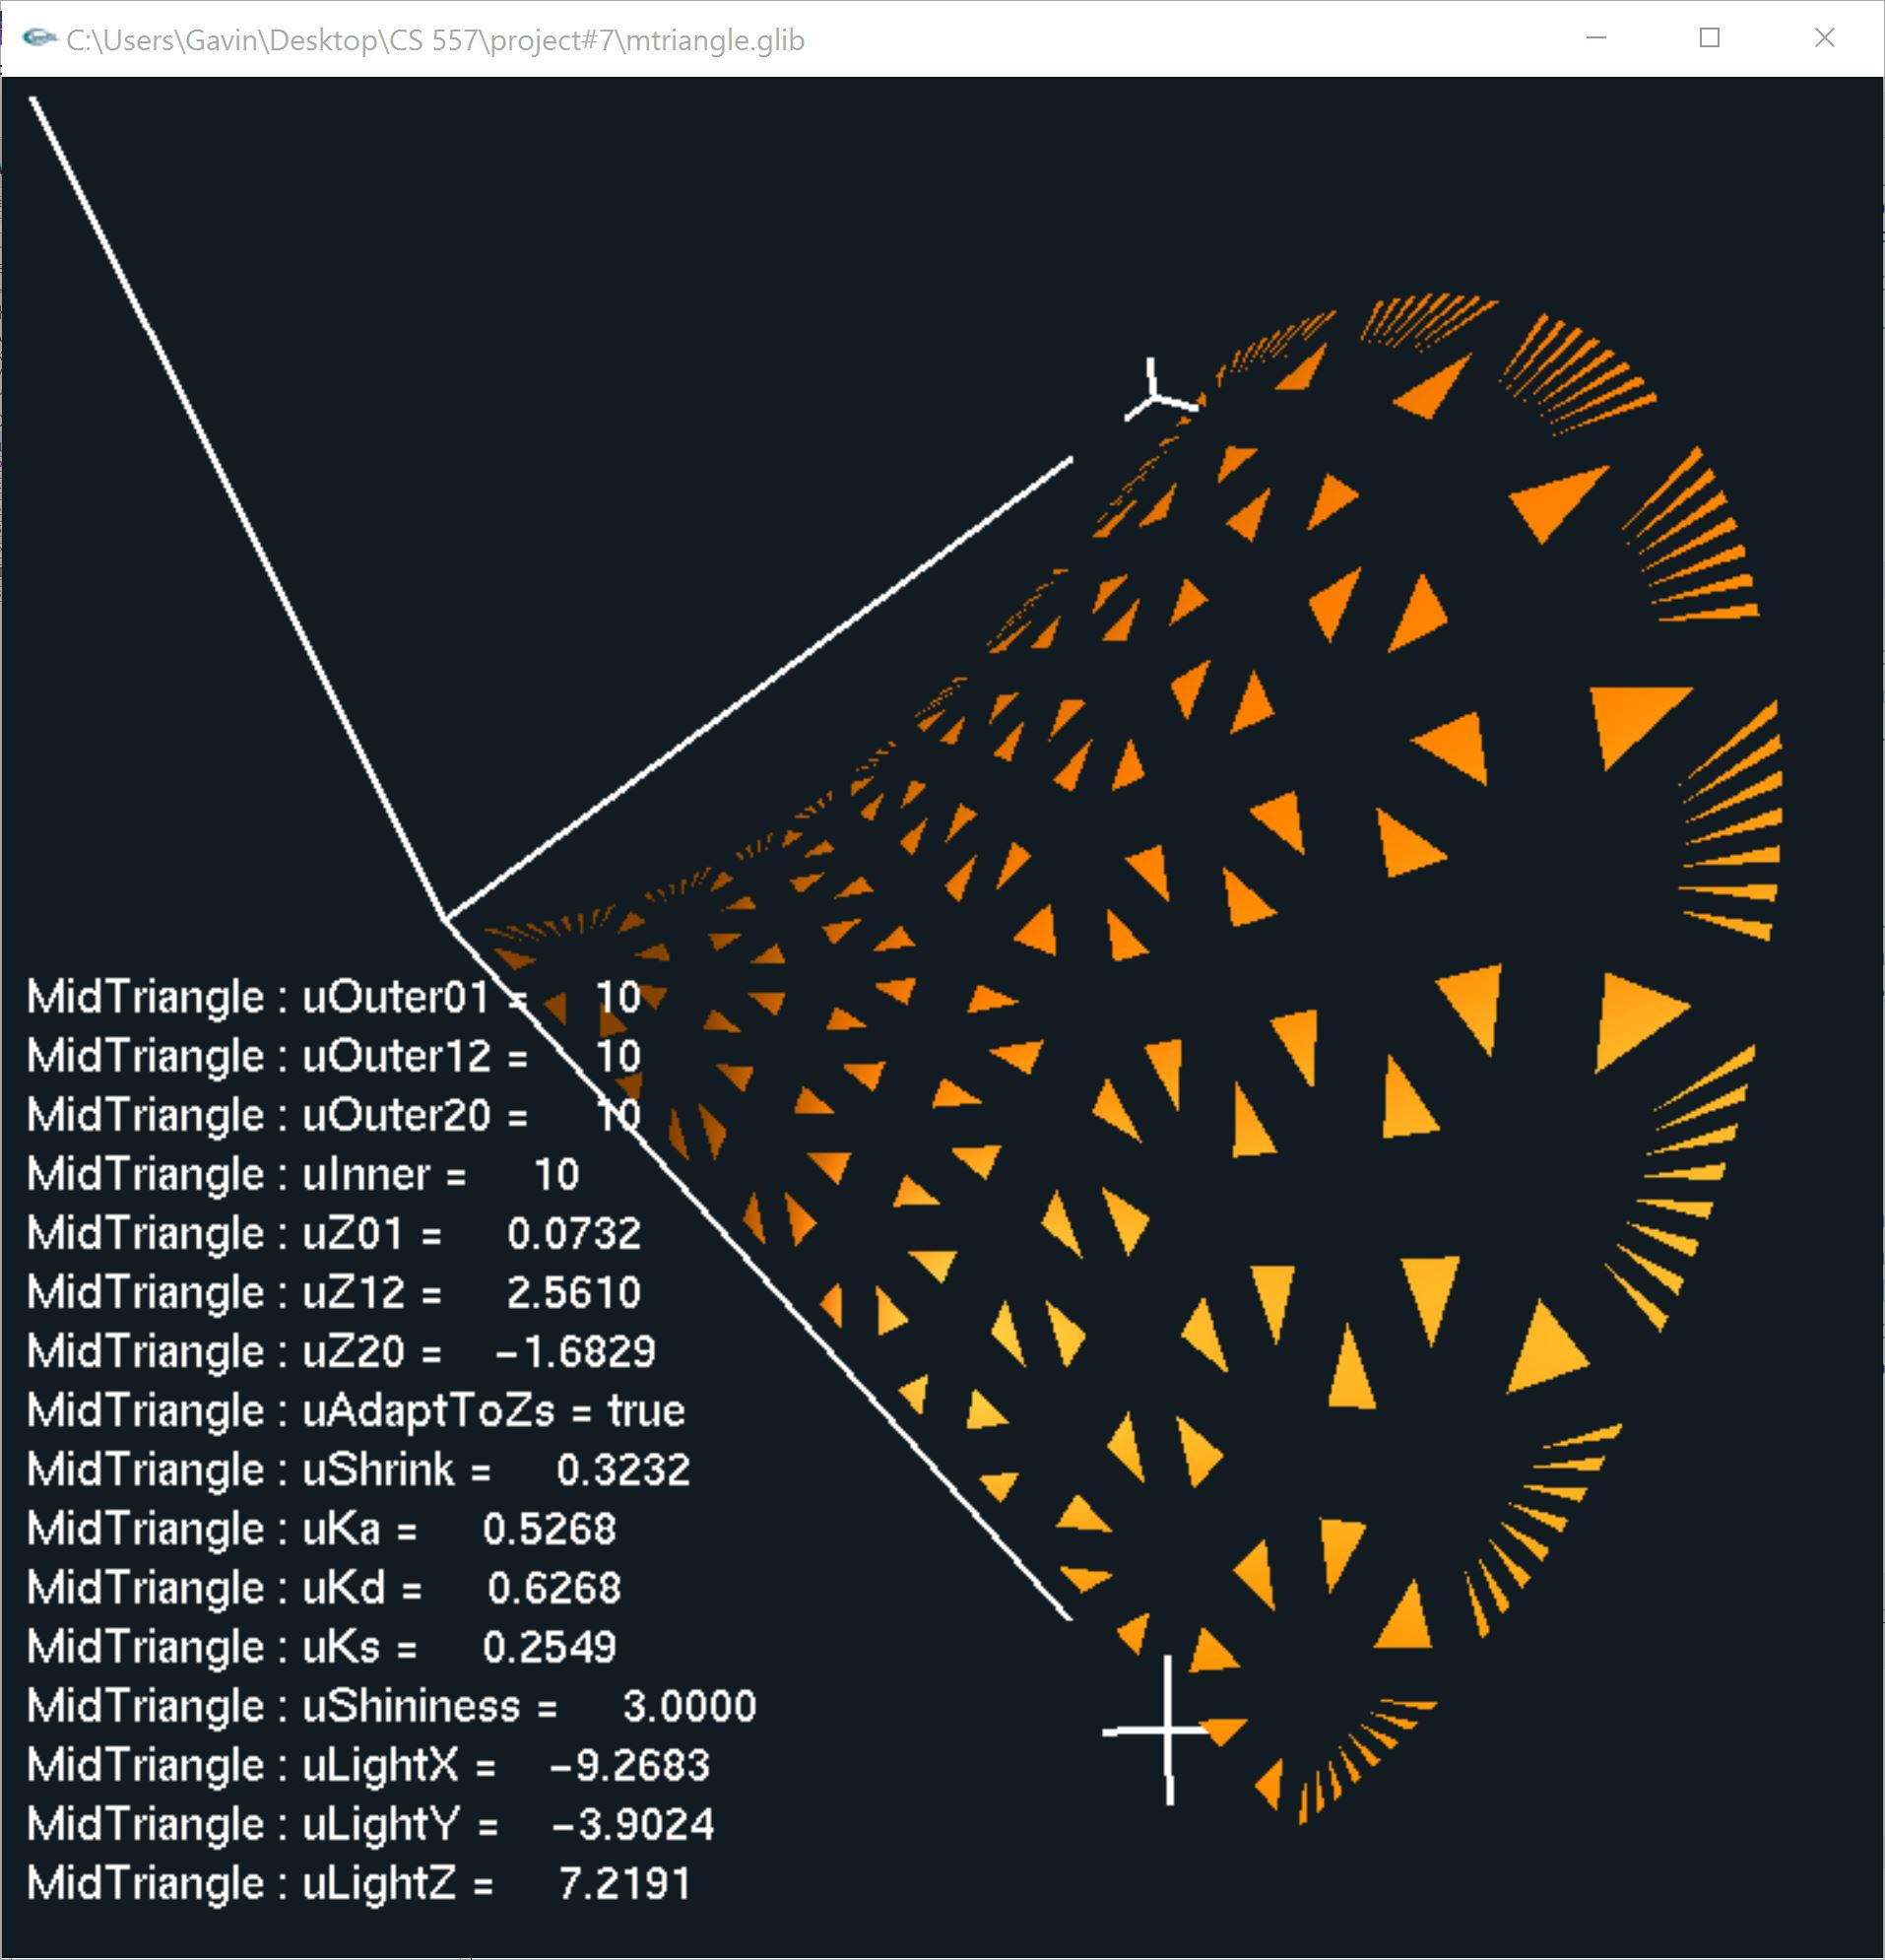
\includegraphics[width=3.2in]{shrink1.jpg}
	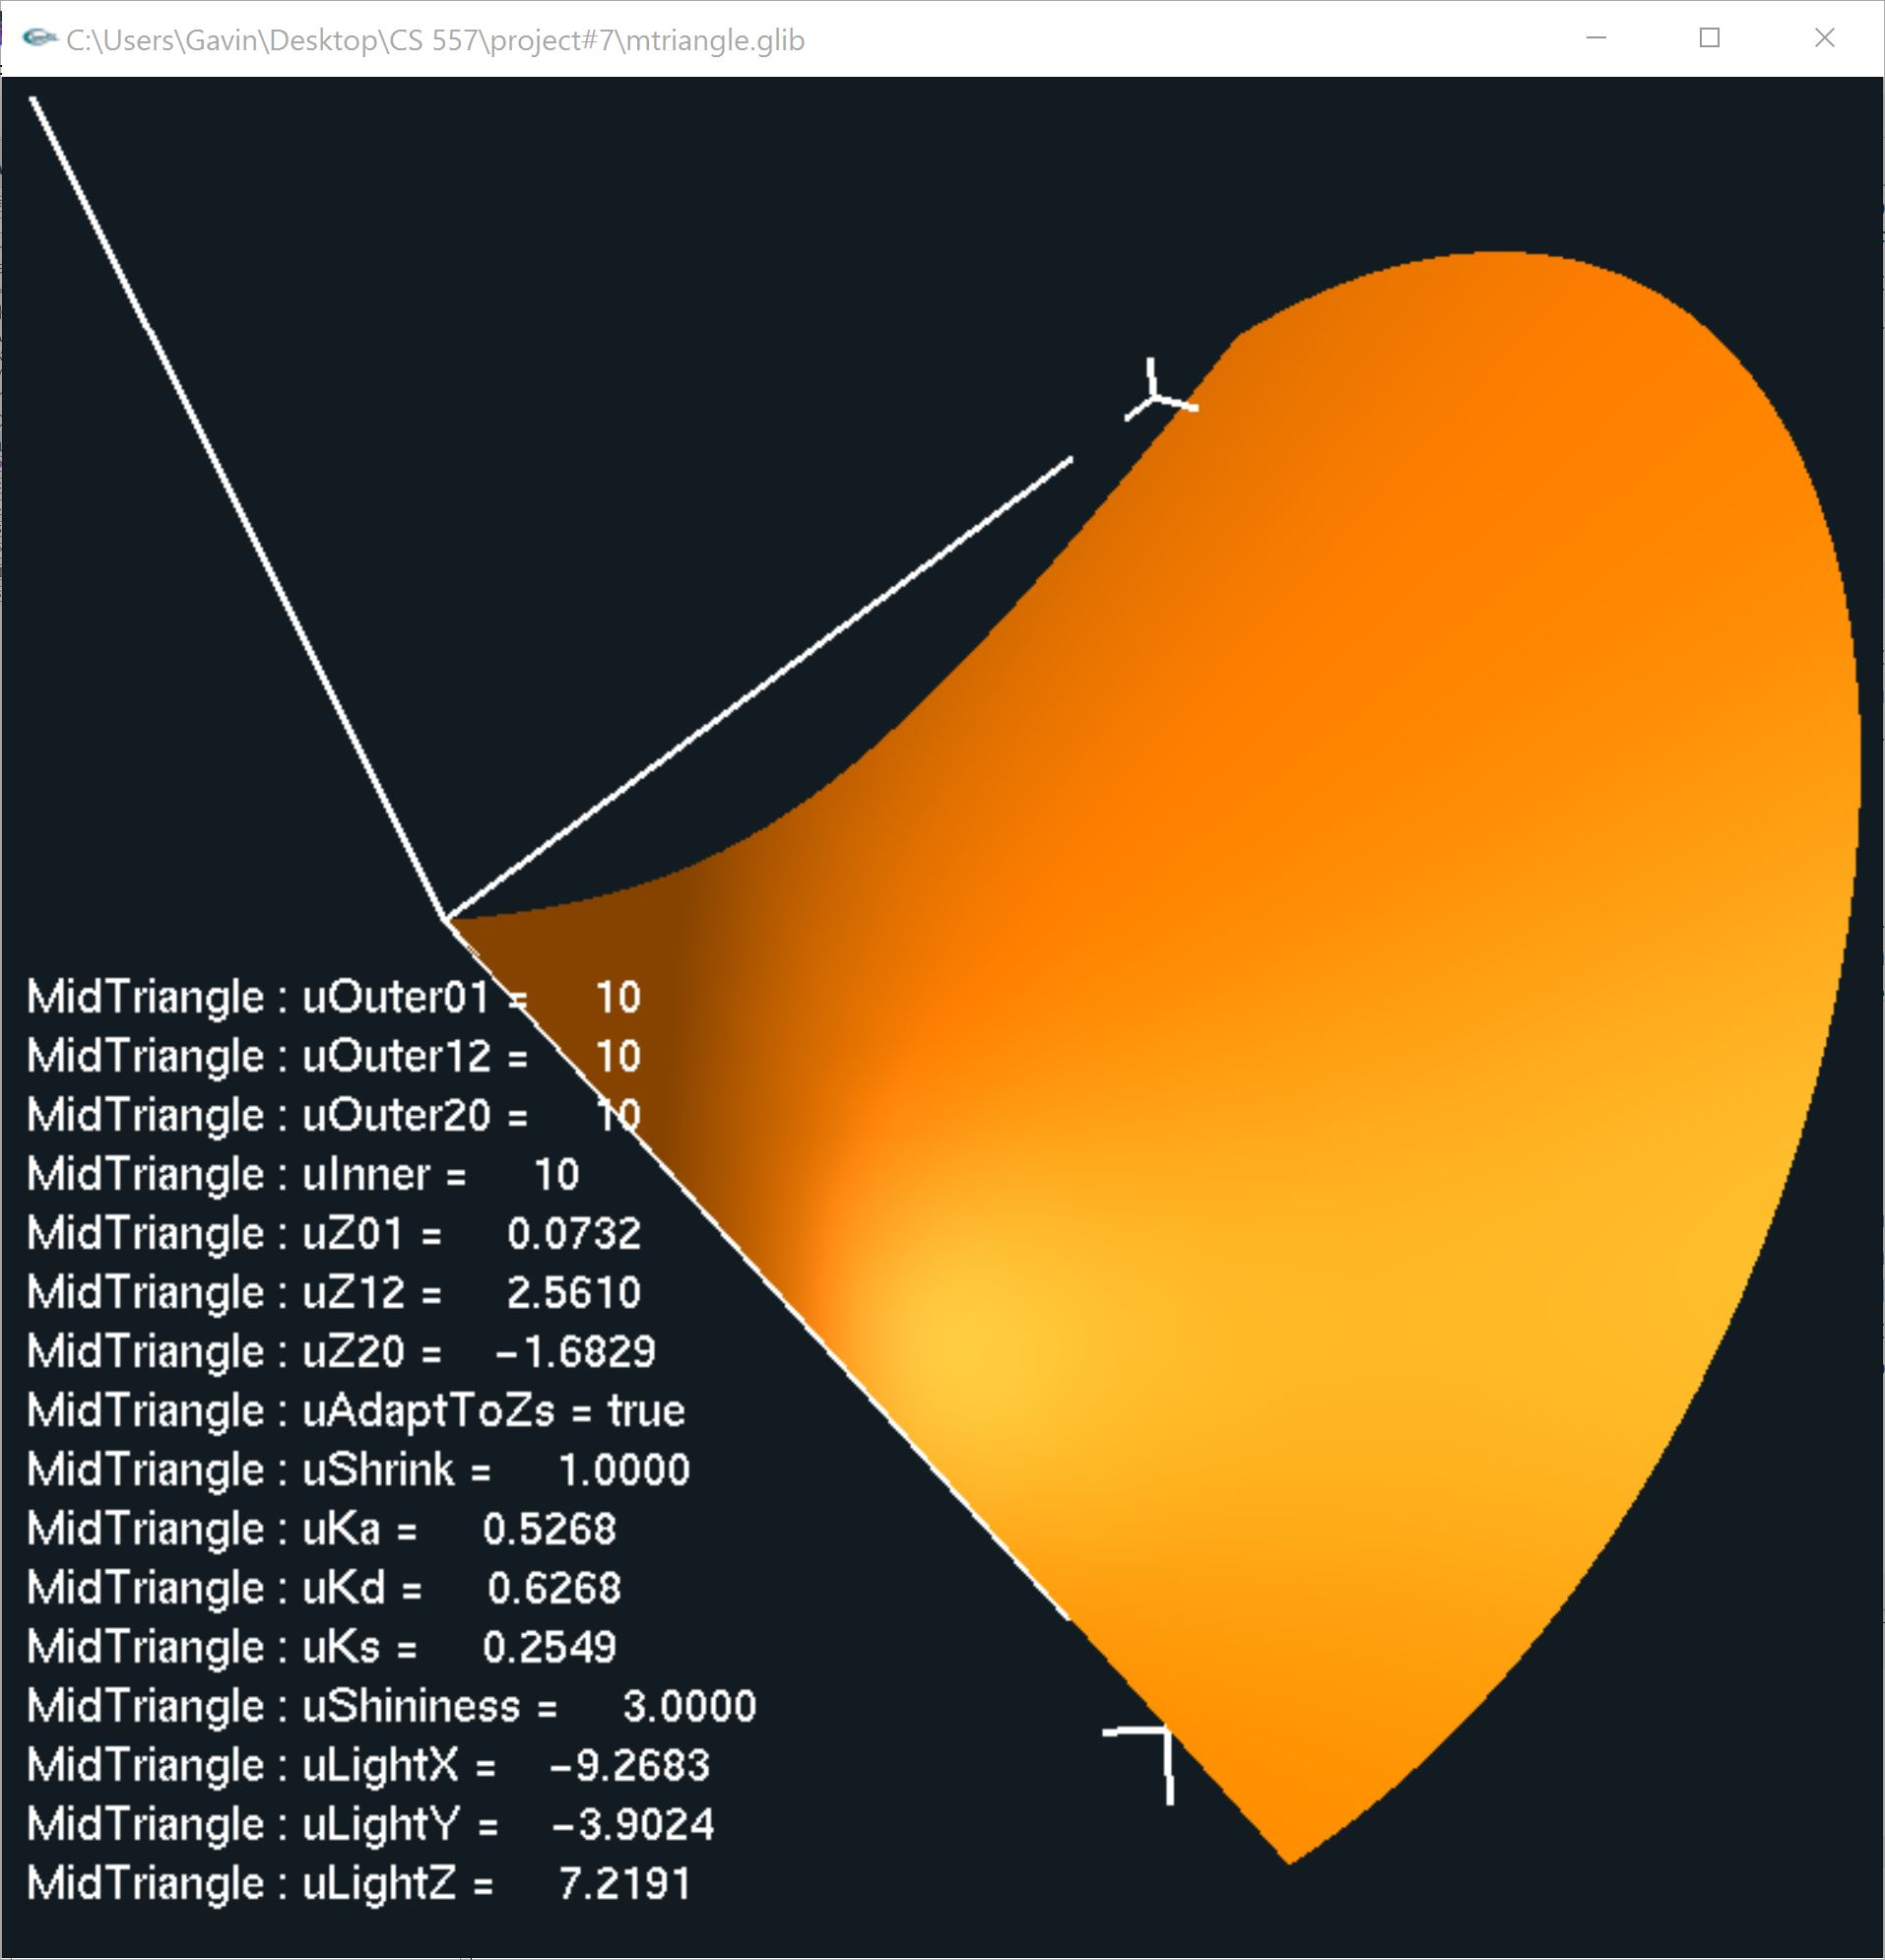
\includegraphics[width=3.2in]{shrink2.jpg}
\end{center}
\section{Summary}
Just as it mentioned in the beginning of the report, this is the last project we have except the final. I've had a lot fun implementing shaders and also learned a lot knowledge and gained a lot experience along the period. I am willing to do the final project well and also do more interesting things with graphics and shaders in my following studying life.
\end{document}